\documentclass[10pt, aspectratio=169]{beamer}
\usetheme{Madrid}
\usecolortheme{whale}
\usepackage{amsmath, amssymb, amsthm}
\usepackage{graphicx}
\usepackage{booktabs}
\usepackage{xcolor}
\usepackage{tikz}
\usepackage{pgfplots}
\pgfplotsset{compat=1.17}
\usepackage{natbib}
\usepackage{bbm}

% Color definitions
\definecolor{aaltoBlue}{RGB}{0,101,189}
\definecolor{aaltoDark}{RGB}{0,50,100}
\definecolor{aaltoRed}{RGB}{179,7,56}
\definecolor{aaltoGreen}{RGB}{0,155,119}
\definecolor{aaltoGray}{RGB}{100,100,100}

% Theme customization
\setbeamercolor{frametitle}{bg=aaltoBlue, fg=white}
\setbeamercolor{title}{fg=white}
\setbeamercolor{titlelike}{fg=aaltoBlue}
\setbeamercolor{structure}{fg=aaltoBlue}
\setbeamercolor{block title}{bg=aaltoBlue, fg=white}
\setbeamercolor{block body}{bg=aaltoBlue!10}
\setbeamercolor{block title alerted}{bg=aaltoRed, fg=white}
\setbeamercolor{block body alerted}{bg=aaltoRed!10}
\setbeamercolor{block title example}{bg=aaltoGreen, fg=white}
\setbeamercolor{block body example}{bg=aaltoGreen!10}
\setbeamertemplate{navigation symbols}{}
\setbeamertemplate{footline}[frame number]
\setbeamerfont{frametitle}{size=\normalsize, series=\bfseries}

% Math shortcuts
\newcommand{\E}{\mathbb{E}}
\newcommand{\G}{\mathcal{G}}
\newcommand{\Cov}{\mathrm{Cov}}
\newcommand{\Var}{\mathrm{Var}}
\newcommand{\sign}{\mathrm{sign}}

\newtheorem{proposition}{Proposition}

\title[Redistributive Peak-Load Pricing]{\textbf{Redistributive Peak-Load Pricing}}
\author[L. Monjoie]{L\'eopold Monjoie}
\institute[Aalto University]{Aalto University \\ \texttt{leopold.monjoie@aalto.fi}}
\date{\today}

%%%%%%%%%%%%%%%%%%%%%%%%%%%%%%%%%%%%%%%%%%%%%%%%%%%%%%%%%%%%%
\begin{document}
%%%%%%%%%%%%%%%%%%%%%%%%%%%%%%%%%%%%%%%%%%%%%%%%%%%%%%%%%%%%%

%-----------------------------------------------------------%
\begin{frame}
\titlepage
\end{frame}

%-----------------------------------------------------------%
\begin{frame}{Overview of contributions}
\begin{block}{Core question}
How should a market designer allocate a scarce, non-storable good across consumers with private information and redistributive objectives?
\end{block}
\vspace{0.3cm}
\textbf{Three contributions:}
\begin{enumerate}
\item \textbf{Redistributive incidence of capacity expansion and redistribution priorities.} Who benefits from a larger $k$ and higher priorities? Depends on two sorting margins and sufficient statistics.
\item \textbf{Optimal tagging rule.} How to rank observable categories in terms of capacity allocation, budget contribution, and redistributive priority. Three rankings governed by distinct primitives.
\item \textbf{Incomplete-information peak-load investment rule.} The informational wedge persists at the optimum under redistributive preferences, unlike the utilitarian case.
\end{enumerate}
\vspace{0.2cm}
\begin{alertblock}{Key observation}
Under redistributive preferences, relying only on a uniform price signal (eg. spot price) \emph{fails} to implement the optimal allocation even when individual transfers are feasible.
\end{alertblock}
\end{frame}

%-----------------------------------------------------------%
\begin{frame}{Motivation: essential goods and the normative tension}
\textbf{Three sectors where this matters:}
\begin{itemize}
\item \textbf{Electricity:} \$2bn annual DWL from flat retail pricing (Hinchberger 2024); 2021 Texas blackout cost \$80--130bn. IEA projects 4,600 GW of new renewable capacity by 2030.
\item \textbf{Transport:} \$269bn annual congestion costs in US urban areas. OECD estimates USD 400 per capita per year in investment needs in high-income cities.
\item \textbf{Health:} COVID-19 vaccine misallocation caused $\approx$ 1.3m direct deaths by end of 2021.
\end{itemize}
\vspace{0.3cm}
\textbf{The fundamental tension:}
\begin{columns}
\begin{column}{0.48\textwidth}
\begin{block}{Classical logic}
Allocate scarce capacity to the \emph{highest WTP} consumers. Finance investment through \emph{scarcity prices}.
\end{block}
\end{column}
\begin{column}{0.48\textwidth}
\begin{alertblock}{Redistributive concern}
Access during shortages and burden of financing should \emph{not} be determined solely by WTP.
\end{alertblock}
\end{column}
\end{columns}
\vspace{0.2cm}
$\Rightarrow$ Allocation of scarce supply and financing of expansion are part of the \emph{same} economic problem.
\end{frame}


%-----------------------------------------------------------%
\begin{frame}{Related literature}
\textbf{Peak-load pricing:} Boiteux (1949), Steiner (1957), Vickrey (1963), Crew \& Kleindorfer (1995). Efficient allocation under complete information. Under utilitarian incomplete information: Spulber (1992), Chao (1987) — complete- and incomplete-information investment rules coincide at the optimum. With redistributive preferences: Leuthold (1976), Diaz (2014), Russo — optimal mechanism departs from the utilitarian benchmark. \textbf{This paper:} full characterization under both redistributive preferences and incomplete information.
\vspace{0.2cm}

\textbf{Redistributive mechanism design:} Pai \& Vohra (2023), G\"unay et al.\ (2024), Dworczak et al.\ (2021), Kang \& Pei (2021, 2024), M\"akimattila (2025), Cremer et al.\ (2002). Closest: Akbarpour et al.\ (2023) — same architecture, but their revenue weight is exogenous. Here the surplus available for redistribution is an \emph{equilibrium object} depending jointly on investment, preferences, and IC rents, giving rise to the capacity-sorting margin.
\vspace{0.2cm}

\textbf{Sufficient statistics:} Saez (2001), Chetty (2010), Kleven (2021). Utility curvature plays the role of demand responsiveness: it governs how capacity is reallocated as $k$ expands and how preference perturbations translate into quantity reallocation.
\vspace{0.2cm}

\textbf{Group-based differentiation:} Akerlof (1978), Cremer et al.\ (2002). Applied to electricity by Borenstein (2012) and Burger (2020); to vaccine allocation by Akbarpour et al.\ (2023) and Pathak et al.\ (2024).
\end{frame}
%-----------------------------------------------------------%
\begin{frame}{Summary of results}
\begin{table}
\small
\begin{tabular}{lll}
\toprule
\textbf{Question} & \textbf{Governing object} & \textbf{Key finding} \\
\midrule
Who benefits from $\uparrow k_i$? & $\E_{(s,i)}^w[uJ \mid s]$ (EuJ) and $R_\theta$ & Non-monotone; sign + regime \\
& & determines winners/losers \\
\midrule
How does $\uparrow \lambda_i$ reshape & $R_\G(\theta) = \Delta\G_i/\G_i$ & Non-monotone; alternating \\
the allocation? & revenue $\Cov_i(R_\theta, R_\G)$ & winner-loser pattern \\
\midrule
Capacity ranking & $\E_i[R_\G(\theta)]$ & Proportional, not absolute \\
across categories & & differences \\
\midrule
Revenue: who contributes? & $\tilde\lambda_i$ (average weight) & Clean separation: $N^+$ vs $N^0$ \\
Revenue: how much? & Both sorting margins & Non-trivial interaction \\
\midrule
Optimal investment rule & $\G_i(\theta)/\tilde\lambda^\ast$ & IC distortion persists at $k^\ast$ \\
& & (unlike utilitarian case) \\
\midrule
Global expansion incidence & $\E_{(s,i)}^w[uJ \mid s]$ vs $I'(k)$ & Convergence vs divergence \\
\bottomrule
\end{tabular}
\end{table}
\end{frame}
%-----------------------------------------------------------%
\begin{frame}{Environment: consumers}
\textbf{Unit mass of consumers}, each characterized by $(i, \theta)$ subject to a common shock $s$.
\vspace{0.2cm}
\begin{itemize}
\item \textbf{Category} $i \in N = \{1,\dots,n\}$: publicly observed, mass $\mu_i > 0$, $\sum_i \mu_i = 1$.
\item \textbf{Type} $\theta \in \Theta_i = [\underline{\theta}_i, \overline{\theta}_i]$: \emph{privately observed}, drawn from $G_i$ with density $g_i > 0$. Independent across consumers.
\item \textbf{Common shock} $s \in S = [\underline{s}, \overline{s}]$: drawn from $F$ with density $f > 0$, observed by all agents.
\end{itemize}
\vspace{0.3cm}
\textbf{Preferences:} consumer of type $\theta$ derives value from quantity $q$ in state $s$:
\[ \theta\, U(q,s) = \theta \int_0^q u(\tilde{q}, s)\, d\tilde{q}, \quad U(0,s)=0 \]
with $u_s > 0$ (higher demand in high states) and $u_q < 0$ (decreasing marginal utility). Transfers are separable, no income effects.
\vspace{0.2cm}
\textbf{Expected surplus} of a consumer receiving $(q_i(\theta,s), t_i(\theta,s))$:
\[ \E_s\!\left[\theta U(q_i(\theta,s),s) - t_i(\theta,s)\right] \]
\end{frame}

%-----------------------------------------------------------%
\begin{frame}{Environment: technology, feasibility, and objective}
\textbf{Technology:} Investment level $k \geq 0$ at cost $I(k)$, $I$ increasing and convex. Zero marginal production cost.
\vspace{0.2cm}
\textbf{Three feasibility constraints:}
\begin{itemize}
\item \textbf{(IR)} $\E_s\!\left[\theta U(q_i(\theta,s),s) - t_i(\theta,s)\right] \geq 0$ for all $\theta \in \Theta_i$.
\item \textbf{(K)} $Q(s) = \sum_i \mu_i \E_i[q_i(\theta,s)] \leq k$ for all $s \in S$.
\item \textbf{(R)} $\sum_i \mu_i \E_{(s,i)}[t_i(\theta,s)] - I(k) \geq 0$.
\end{itemize}
\vspace{0.3cm}
\textbf{Planner's objective:} weighted expected sum of consumer surpluses with welfare weights $\lambda_i(\theta) \geq 0$:
\[ \sum_i \mu_i\, \E_{(s,i)}\!\left[\lambda_i(\theta)\bigl(\theta U(q_i(\theta,s),s) - t_i(\theta,s)\bigr)\right] \]
where $\tilde{\lambda}_i := \E_i[\lambda_i(\theta)]$ is the average weight in category $i$.
\vspace{0.2cm}
\begin{block}{Timing}
(i) Consumers learn $\theta$. (ii) Designer chooses $k$. (iii) Mechanism $(q_i, t_i)$ proposed. (iv) Shock $s$ realized, allocations implemented.
\end{block}
\end{frame}

%-----------------------------------------------------------%
\begin{frame}{Mechanism: revelation principle and IC representation 1}
By the revelation principle, focus on \textbf{direct mechanisms}. IC in expectation requires for all $\theta, \hat{\theta} \in \Theta_i$:
\[ \E_s\!\left[\theta U(q_i(\theta,s),s) - t_i(\theta,s)\right] \geq \E_s\!\left[\theta U(q_i(\hat{\theta},s),s) - t_i(\hat{\theta},s)\right] \tag{IC$^\times$} \]
\vspace{0.2cm}
\textbf{Envelope representation:} Under (IC$^\times$), the expected surplus satisfies
\[ \E CS_i(\theta) = \E\underline{CS}_i + \int_{\underline{\theta}_i}^{\theta} \E_s\!\left[U(q_i(\tilde{\theta},s),s)\right] d\tilde{\theta} \tag{$\E CS_i$} \]
for some boundary term $\E\underline{CS}_i \geq 0$.

\end{frame}

%-----------------------------------------------------------%
\begin{frame}{Mechanism: revelation principle and IC representation 2}

\vspace{0.2cm}
\begin{alertblock}{Note on IC}
IC in expectation is weaker than pointwise IC. At the optimum, Assumption Int ensures that $\G_i(\theta)$ is non-decreasing, which implies pointwise IC is satisfied. Imposing IC in expectation is therefore without loss at the optimum.
\end{alertblock}
\vspace{0.2cm}
\textbf{Analysis proceeds in three steps:}
\begin{enumerate}
\item Optimal \emph{within-category} mechanism for given $(k_i, I_i)$.
\item Optimal \emph{across-category} allocation of $(k_i, I_i)$.
\item Optimal \emph{investment level} $k^\ast$.
\end{enumerate}
\end{frame}

%-----------------------------------------------------------%
\begin{frame}{Virtual surplus primitives 1}
\textbf{Key objects:} for category $i$ and type $\theta$,
\begin{columns}
\begin{column}{0.48\textwidth}
\begin{block}{Inverse hazard rate}
\[ \gamma_i(\theta) := \frac{1 - G_i(\theta)}{g_i(\theta)} \]
Measures the ``leakage'' cost: serving type $\theta$ forces the designer to concede rent to all higher types.
\end{block}
\end{column}
\begin{column}{0.48\textwidth}
\begin{block}{Virtual surplus}
\[ J_i(\theta) := \theta - \gamma_i(\theta) \]
Net revenue extractable from type $\theta$ after accounting for upward rent spillovers. \textbf{Can be negative.}
\end{block}
\end{column}
\end{columns}

\end{frame}

%-----------------------------------------------------------%
\begin{frame}{Virtual surplus primitives 2}
\textbf{Key objects:} for category $i$ and type $\theta$,
\begin{block}{IC-adjusted redistributive term}
\[ \Lambda_i(\theta) := \gamma_i(\theta)\, \E_i\!\left[\lambda_i(\tilde{\theta}) \mid \tilde{\theta} \geq \theta\right] \]
The social value of rents flowing upward to types $\tilde\theta > \theta$ when type $\theta$ receives a marginal unit, evaluated at their average welfare weight.
\end{block}
\vspace{0.2cm}
\begin{block}{Total social return from allocating to type $\theta$}
\[ \Gamma_i(\theta) := \tilde{\lambda}_i J_i(\theta) + \Lambda_i(\theta) \]
Combines: \textbf{(i)} revenue channel $\tilde{\lambda}_i J_i(\theta)$ (net revenue valued at average weight), and \textbf{(ii)} redistributive channel $\Lambda_i(\theta)$ (social value of upward rents).
\end{block}
\end{frame}

%-----------------------------------------------------------%
\begin{frame}{Lemma: Virtual surplus representation}
\begin{lemma}[Virtual surplus representation]
The designer's program can be expressed as:
\[ \max_{q_i(\theta,s),\, \E\underline{CS}_i} \sum_i \mu_i \left\{ \tilde{\lambda}_i\, \E\underline{CS}_i + \E_{(s,i)}\!\left[\Lambda_i(\theta)\, U(q_i(\theta,s),s)\right] \right\} \tag{CS} \]
subject to the capacity constraint \emph{(K)}, participation $\E\underline{CS}_i \geq 0$, and
\[ \sum_i \mu_i \left(\E_{(s,i)}\!\left[U(q_i(\theta,s),s)\, J_i(\theta)\right] - \E\underline{CS}_i\right) - I(k) \geq 0. \tag{R} \]
\end{lemma}
\vspace{0.2cm}
\textbf{Decomposition:} Because the objective and constraints are separable across categories (except through aggregate capacity and revenue), the problem decomposes into:
\begin{enumerate}
\item An \textbf{across-category} allocation of $(k_i, I_i)$ satisfying $\sum_i \mu_i k_i = k$ and $\sum_i \mu_i I_i = I(k)$.
\item For each $i$, a \textbf{within-category} problem that determines $q_i(\theta,s)$ given $(k_i, I_i)$.
\end{enumerate}
\end{frame}

%-----------------------------------------------------------%
\begin{frame}{Optimal within-category allocation: the combined constraint}
Fix $(k_i, I_i)$. Since slack in the revenue requirement can be rebated lump-sum, \textbf{the revenue constraint binds at the optimum}: $\E_{(s,i)}[t_i(\theta,s)] = I_i$.
\vspace{0.2cm}
Substituting the envelope representation into the binding revenue constraint and integrating by parts yields the single combined constraint:
\[ \E\underline{CS}_i = \E_{(s,i)}\!\left[U(q_i(\theta,s),s)\, J_i(\theta)\right] - I_i \tag{$\E\underline{CS}_i$} \]
Substituting into the objective, the within-category problem becomes:
\[ \max_{q_i(\theta,s)}\; \E_{(s,i)}\!\left[\Gamma_i(\theta)\, U(q_i(\theta,s),s) - \tilde{\lambda}_i I_i\right] \tag{CS$_i$} \]
subject to
\[ \E_{(s,i)}\!\left[U(q_i(\theta,s),s)\, J_i(\theta)\right] - I_i \geq 0 \tag{IR-R$_i$} \]
\[ \E_i\!\left[q_i(\theta,s)\right] \leq k_i \quad \forall s \tag{K$_i$} \]
where $\Gamma_i(\theta) = \tilde{\lambda}_i J_i(\theta) + \Lambda_i(\theta)$ is the total social return from allocating to type $\theta$.
\end{frame}

%-----------------------------------------------------------%
\begin{frame}{Lemma: Off-peak and on-peak allocation 1}
Let $\beta_i \geq 0$ and $\varepsilon_i(s) \geq 0$ denote the multipliers on (IR-R$_i$) and (K$_i$). Define the \textbf{effective social weight}:
\[ \G_i(\theta) := \Gamma_i(\theta) + J_i(\theta)\,\beta_i = (\tilde{\lambda}_i + \beta_i)\,J_i(\theta) + \Lambda_i(\theta) \]
\begin{lemma}[Off-peak and on-peak allocation]
Under Assumption Int ($\G_i(\theta) > 0$ and non-decreasing), the allocation is:
\[ u(q_i(\theta,s),s) = 0 \quad s \in S_i, \qquad u(q_i(\theta,s),s)\,\G_i(\theta) = \varepsilon_i(s) \quad s \in T_i \tag{SB-S/T} \]
where $S_i = [\underline{s}, s_i)$ and $T_i = [s_i, \overline{s}]$ with $\E_i[q_i(\theta,s_i)] = k_i$.
\end{lemma}
\end{frame}
%-----------------------------------------------------------%
\begin{frame}{Lemma: Off-peak and on-peak allocation 2}

\begin{columns}
\begin{column}{0.48\textwidth}
\begin{block}{Off-peak ($s \in S_i$)}
$\varepsilon_i(s) = 0$, constraint slack. Allocation independent of $\theta$. Automatic monotonicity.
\end{block}
\end{column}
\begin{column}{0.48\textwidth}
\begin{block}{On-peak ($s \in T_i$)}
$\varepsilon_i(s) > 0$, capacity binds. Type $\theta$ with higher $\G_i(\theta)$ receives \emph{more} allocation. Scarcity rent $\varepsilon_i(s)$ equalized in aggregate.
\end{block}
\end{column}
\end{columns}
\vspace{0.2cm}
\textbf{Key:} $\G_i(\theta)$ is an \emph{equilibrium object}. When $J_i(\theta) > 0$, a looser budget ($\beta_i$ falls) reduces the premium on revenue-generating types.
\end{frame}
%-----------------------------------------------------------%
\begin{frame}{The capacity-sorting margin}
\textbf{Two objects govern the analysis:}
\begin{columns}
\begin{column}{0.48\textwidth}
\begin{block}{Demand responsiveness}
\[ R_q(\theta) := -\frac{u(q_i(\theta,s),s)}{u_q(q_i(\theta,s),s)} \geq 0 \]
Governed by \emph{curvature of demand}. Determines how a marginal increase in $k_i$ is distributed across types at the optimal allocation.
\end{block}
\end{column}
\begin{column}{0.48\textwidth}
\begin{block}{Revenue sorting}
\[ R_\theta(\theta) := \frac{J_i(\theta)}{\G_i(\theta)} \]
Governed by \emph{type distribution and redistributive preferences}. Determines how marginal virtual surplus $u(q_i,s)J_i(\theta)$ varies across types.
\end{block}
\end{column}
\end{columns}
\vspace{0.3cm}
\begin{alertblock}{The capacity-sorting margin (EuJ)}
\[ \E_{(s,i)}^w[uJ \mid s] := \E_s\!\left[\E_i^w[uJ \mid s]\, \mathbf{1}_{\{s \in T_i\}}\right] \]
Decomposition into \textbf{average} and \textbf{sorting} effects:
\[ \E_i\!\left[R_\theta(\theta) R_q(\theta)\right] = \underbrace{\E_i[R_\theta]\, \E_i[R_q]}_{\text{average effect}} + \underbrace{\Cov_i(R_\theta, R_q)}_{\text{sorting effect}} \tag{signEuJ} \]
\end{alertblock}
\vspace{0.1cm}
\textbf{Interpretation:} The sorting effect is adverse when additional capacity is tilted toward types with \emph{lower} marginal virtual surplus. If $\Cov_i(R_\theta, R_q) < 0$, expanding capacity reduces the designer's revenue margin.
\end{frame}

%-----------------------------------------------------------%
\begin{frame}{Single-crossing of the capacity-sorting margin1}
\begin{lemma}[Single-crossing, Lemma SC-dir]
Assume $\theta \mapsto R_\theta(\theta)$ is monotone and $R_q(\theta)$ has log-monotone differences in $(\theta, k_i)$. Then the map $k_i \mapsto \E_{(s,i)}^w[uJ \mid s]$ is \textbf{single-crossing} in $k_i$.
\end{lemma}
\vspace{0.2cm}
\textbf{Direction of crossing:}
\begin{itemize}
\item Crosses from $+$ to $-$: when $R_\theta$ increasing and $R_q$ log-submodular, OR when $R_\theta$ decreasing and $R_q$ log-supermodular.
\item Crosses from $-$ to $+$: in the two remaining cases.
\end{itemize}
\end{frame}
%-----------------------------------------------------------%
\begin{frame}{Single-crossing of the capacity-sorting margin 2}
\textbf{Primitive foundations:}
\begin{itemize}
\item $\sign(R_q'(\theta)) = -\sign\!\left((u_q)^2 - u\cdot u_{qq}\right)$: $R_q' < 0$ for linear/quadratic demand, $R_q' > 0$ for CES/isoelastic.
\item $\sign(R_\theta'(\theta)) = \sign(J_i(\theta))\cdot\sign\!\left(\frac{J_i'(\theta)}{J_i(\theta)} - \frac{\Lambda_i'(\theta)}{\Lambda_i(\theta)}\right)$: depends on whether virtual surplus grows faster than the IC term.
\end{itemize}
\vspace{0.2cm}
\begin{block}{Special case: CARA preferences}
$u(q,s) = v(s)\exp(-\alpha q)$ implies $R_q = 1/\alpha$ is constant. Additional capacity distributed across types in proportions determined solely by welfare weights.
\end{block}
\end{frame}
%-----------------------------------------------------------%
\begin{frame}{Theorem: redistributive incidence of capacity expansion}
\begin{theorem}[Redistributive effects of capacity expansion]
Fix category $i$, budget $I_i > 0$. Under Assumptions Monot. and Multi.:

\textbf{IR-unconstrained.} If $\E_{(s,i)}^w[uJ \mid s] > 0$: every type gains from $\uparrow k_i$. If $\E_{(s,i)}^w[uJ \mid s] < 0$: at most one cutoff $\tilde\theta_i$ exists; types below lose, types above gain.

\textbf{IR-constrained.} The lowest type $\underline{\theta}_i$ always lies on the boundary. A second cutoff $\tilde\theta_i \in (\underline{\theta}_i, \overline{\theta}_i)$ may exist, and when it does:
\begin{itemize}
\item[(i)] If $\E_{(s,i)}^w[uJ \mid s] > 0$: surplus $\uparrow$ for $\theta \in (\underline{\theta}_i, \tilde\theta_i)$, $\downarrow$ for $\theta \geq \tilde\theta_i$.
\item[(ii)] If $\E_{(s,i)}^w[uJ \mid s] < 0$: surplus $\downarrow$ for $\theta \in (\underline{\theta}_i, \tilde\theta_i)$, $\uparrow$ for $\theta \geq \tilde\theta_i$.
\end{itemize}
If $R_\theta(\theta)$ is decreasing, all inequalities are reversed.
\end{theorem}
\vspace{0.2cm}
\textbf{Economic mechanism:}
\begin{itemize}
\item IR-unconstrained: expansion operates through the \emph{boundary term} $\E\underline{CS}_i$. The sign of (EuJ) determines whether the common surplus component increases.
\item IR-constrained: expansion operates through the \emph{optimal allocation} $q_i(\theta,s)$. The endogenous response of $\beta_i$ creates type-dependent effects via $R_\theta(\theta)$.
\end{itemize}
\end{frame}

%-----------------------------------------------------------%
\begin{frame}{Implementation regime geometry}
\begin{figure}
\centering
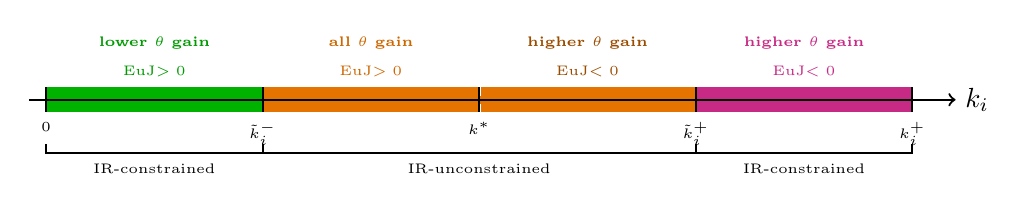
\begin{tikzpicture}[x=1.1cm, y=0.8cm]
\fill[green!70!black]   (0,-0.2) rectangle (2.5,0.2);
\fill[orange!90!black]  (2.5,-0.2) rectangle (5.0,0.2);
\fill[orange!90!black]  (5.0,-0.2) rectangle (7.5,0.2);
\fill[magenta!80!black] (7.5,-0.2) rectangle (10.0,0.2);
\draw[white, dashed, line width=1pt] (5.0,-0.2) -- (5.0,0.2);
\draw[thick] (0,-0.7) -- (0,-0.85) -- (2.5,-0.85) -- (2.5,-0.7);
\draw[thick] (2.5,-0.7) -- (2.5,-0.85) -- (7.5,-0.85) -- (7.5,-0.7);
\draw[thick] (7.5,-0.7) -- (7.5,-0.85) -- (10,-0.85) -- (10,-0.7);
\node[font=\tiny] at (1.25,-1.1) {IR-constrained};
\node[font=\tiny] at (5.0,-1.1)  {IR-unconstrained};
\node[font=\tiny] at (8.75,-1.1) {IR-constrained};
\node[font=\tiny, green!60!black]   at (1.25,0.45) {EuJ$>0$};
\node[font=\tiny, orange!80!black]  at (3.75,0.45) {EuJ$>0$};
\node[font=\tiny, orange!60!black]  at (6.25,0.45) {EuJ$<0$};
\node[font=\tiny, magenta!80!black] at (8.75,0.45) {EuJ$<0$};
\node[font=\tiny\bfseries, green!60!black]   at (1.25,0.9) {lower $\theta$ gain};
\node[font=\tiny\bfseries, orange!80!black]  at (3.75,0.9) {all $\theta$ gain};
\node[font=\tiny\bfseries, orange!60!black]  at (6.25,0.9) {higher $\theta$ gain};
\node[font=\tiny\bfseries, magenta!80!black] at (8.75,0.9) {higher $\theta$ gain};
\draw[->, thick] (-0.2,0) -- (10.5,0);
\node[right] at (10.5,0) {$k_i$};
\foreach \x/\lbl in {0/$0$, 2.5/$\tilde{k}_i^-$, 5/$k^\ast$, 7.5/$\tilde{k}_i^+$, 10/$k_i^+$}{
\draw[thick] (\x,0.2) -- (\x,-0.2);
\node[below, font=\tiny] at (\x,-0.2) {\lbl};
}
\end{tikzpicture}
\end{figure}
\vspace{-0.1cm}
\textbf{Key takeaways:}
\begin{itemize}
\item The redistributive effect of a capacity expansion is \emph{not invariant} to the installed level $k_i$. The same marginal expansion can be progressive at low $k_i$ and regressive at high $k_i$.
\item The transition between regimes is governed by the single-crossing of (EuJ): when (EuJ) crosses from $+$ to $-$, the boundary term $\E\underline{CS}_i$ is single-peaked, generating the intermediate IR-unconstrained window.
\item \textbf{Policy implication:} knowing the sign of (EuJ) at current capacity is sufficient to determine who wins and loses from a marginal expansion.
\end{itemize}
\end{frame}

%-----------------------------------------------------------%
\begin{frame}{Appendix figure: redistribution\_marg\_k\_uniform}

\begin{figure}
    \centering
    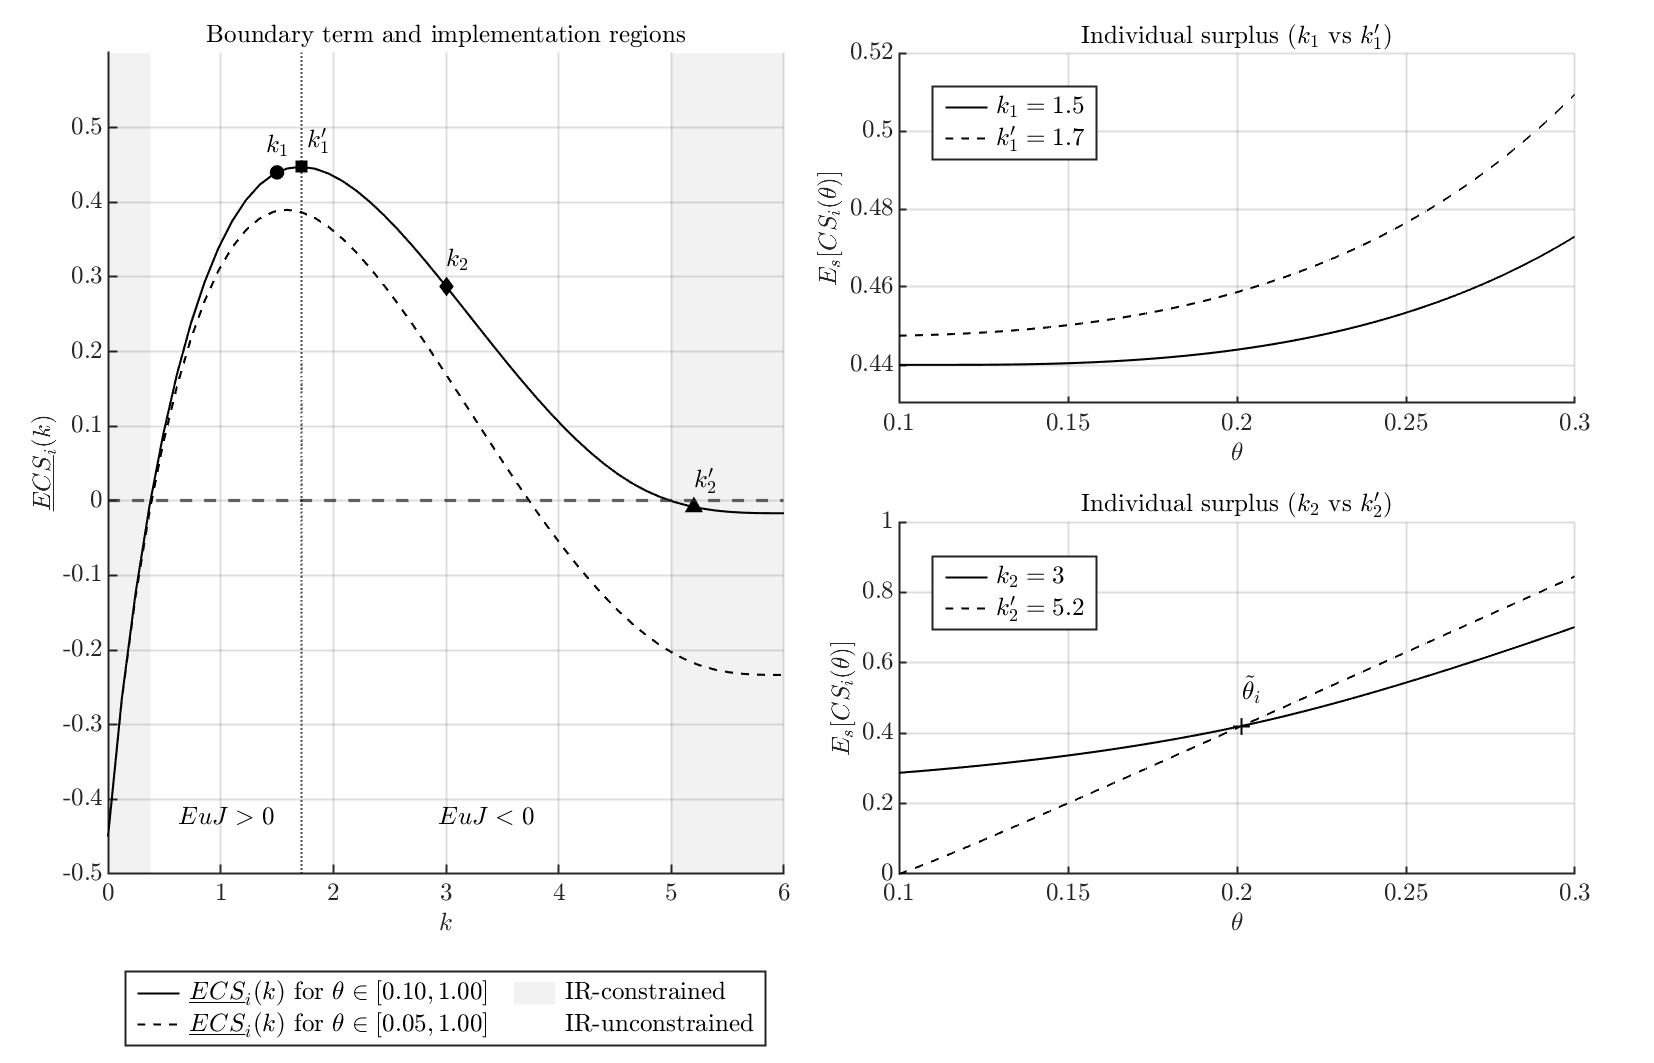
\includegraphics[width=0.8\linewidth]{figure/redistribution_marg_k_uniform.png}
\end{figure}

\end{frame}

%-----------------------------------------------------------%
\begin{frame}{The preference-sorting margin 1 }
Now ask the reverse question: holding $k_i$ fixed, how does a \emph{change in redistributive preferences} reshape the optimal allocation?
\vspace{0.2cm}
\textbf{Perturbation:} $\Delta\lambda_i(\theta)$. The induced change in the effective social weight is:
\[ \Delta\G_i(\theta) = J_i(\theta)(\Delta\tilde{\lambda}_i + \Delta\beta_i) + \Delta\Lambda_i(\theta) \]
\begin{alertblock}{The preference-sorting margin}
\[ R_\G(\theta) := \frac{\Delta\G_i(\theta)}{\G_i(\theta)} \]
Measures how the perturbation tilts the effective weight of type $\theta$ \emph{relative to the baseline allocation}. This is the object that determines the reallocation, not the absolute change $\Delta\G_i(\theta)$.
\end{alertblock}
\end{frame}
%-----------------------------------------------------------%
\begin{frame}{The preference-sorting margin 2}

\begin{lemma}[Preference shifts and effective social weights]\label{lem:preferenceorder}
Consider a weight function $\lambda_i(\theta)$ and its perturbation $\lambda_i^\Delta(\theta)$, with $\Delta\lambda_i(\theta):=\lambda_i^\Delta(\theta)-\lambda_i(\theta)$ and $\Delta\G_i(\theta):=\G_i^\Delta(\theta)-\G_i(\theta)$. Suppose $\G_i(\theta),\G_i^\Delta(\theta)>0$ for all $\theta\in[\underline{\theta}_i,\overline{\theta}_i]$. Define:
\[
m_i(\theta) = \frac{\lambda_i^\Delta(\theta)}{\lambda_i(\theta)}, \qquad c_\Lambda:=\frac{\tilde\lambda_i^\Delta}{\tilde\lambda_i},
\qquad
c_{\G}:=\frac{\tilde\lambda_i^\Delta+\beta_i^\Delta}
{\tilde\lambda_i+\beta_i}.
\]
If $m_i(\theta)$ is increasing on $[\underline{\theta}_i,\overline{\theta}_i]$, then for $\theta\in[\underline{\theta}_i,\overline{\theta}_i]$,
\[
\frac{\Lambda_i^{\Delta\,\prime}(\theta)}{\Lambda_i^\Delta(\theta)} \;\ge\; (\text{resp.} \le) \; \frac{\Lambda_i^{\prime}(\theta)}{\Lambda_i(\theta)}.
\]
Moreover, if $1\le c_{\G}\le c_\Lambda$ (resp. $c_\Lambda\le c_{\G}\le 1$), then for all $\theta\in[\underline{\theta}_i,\overline{\theta}_i]$, $\Delta\G_i(\theta)\ge(\text{resp. }\le)0$. In particular, if either $\beta_i=\beta_i^\Delta=0$ or $\beta_i^\Delta+\tilde\lambda_i^\Delta=\beta_i+\tilde\lambda_i$, then the condition reduces to $\tilde\lambda_i^\Delta\ge (\text{resp. }\le)\tilde\lambda_i$.
\end{lemma}

\end{frame}
%-----------------------------------------------------------%
\begin{frame}{Lemma: reallocation under preference perturbations}
\begin{lemma}[Reallocation under preference perturbations]
Fix category $i$ and allocation $(k_i, I_i)$. For any local perturbation $\Delta\lambda_i(\theta)$ and any allocation regime, in every on-peak state $s \in T_i$:
\[ \Delta q_i(\theta,s) = R_q(\theta)\!\left(R_\G(\theta) - \E_i^w\!\left[R_\G \mid s\right]\right) \]
\end{lemma}
\vspace{0.2cm}
\textbf{Interpretation:} Type $\theta$ receives \emph{more} quantity if and only if its proportional change in effective social weight \emph{exceeds} the capacity-weighted average.
\vspace{0.2cm}
\textbf{Two implications:}
\begin{enumerate}
\item The equilibrium adjustment in the scarcity rent satisfies $\Delta\varepsilon_i(s)/\varepsilon_i(s) = \E_i^w[R_\G \mid s]$: the proportional change in the scarcity rent equals the weighted average of $R_\G$ across types.
\item Since capacity is fixed, the reallocation is \textbf{zero-sum} across types within each binding state: $\E_i[\Delta q_i(\theta,s)] = 0$ for each $s \in T_i$.
\end{enumerate}
\vspace{0.2cm}
\begin{alertblock}{Critical observation}
What drives the response is the \emph{proportional} change $R_\G(\theta)$, not the absolute change $\Delta\G_i(\theta)$. This is the source of non-monotonicity in the surplus effects.
\end{alertblock}
\end{frame}

%-----------------------------------------------------------%
\begin{frame}{Non-monotone reallocation: Proposition rprefreallocation}
\begin{lemma}[Non-monotone reallocation]
Assume $R_\G(\theta)$ is not a.e.\ constant.

\textbf{(i)} Under the IR-unconstrained allocation, $\Delta q_i(\cdot,s)$ is not monotone for any perturbation. Under IR-constrained, the same holds when $|\Delta\tilde\lambda_i|$ is sufficiently small.

\textbf{(ii)} Under mean-preserving perturbation ($\Delta\tilde\lambda_i = 0$): the cutoff set $\{\theta : \Delta q_i(\theta,s)=0\}$ contains at least two elements $\theta_- \leq \theta_+$, and:
\begin{itemize}
\item If $\Delta\G_i(\theta) \geq 0$ for all $\theta$: $\Delta q_i(\theta,s) \leq 0$ for $\theta \in [\underline\theta_i, \theta_-) \cup (\theta_+, \overline\theta_i]$.
\item If $\Delta\G_i(\theta) \leq 0$ for all $\theta$: $\Delta q_i(\theta,s) \geq 0$ for $\theta \in [\underline\theta_i, \theta_-) \cup (\theta_+, \overline\theta_i]$.
\end{itemize}
\end{lemma}
\vspace{0.2cm}
\textbf{Key insight from the proof:} At both endpoints $\underline\theta_i$ and $\overline\theta_i$, under IR-unconstrained allocation with $\beta_i = 0$:
\[ \G_i(\underline\theta_i) = \underline\theta_i\tilde\lambda_i, \quad \G_i(\overline\theta_i) = \overline\theta_i\tilde\lambda_i \quad \Rightarrow \quad R_\G(\underline\theta_i) = R_\G(\overline\theta_i) = \frac{\Delta\tilde\lambda_i}{\tilde\lambda_i} \]
Even if $\Delta\G_i(\underline\theta_i) \neq \Delta\G_i(\overline\theta_i)$, the \emph{proportional} change is identical at both endpoints. The boundary types necessarily move in the \emph{opposite} direction from the interior reallocation under mean-preserving perturbations.
\end{frame}

%-----------------------------------------------------------%
\begin{frame}{Proposition: surplus effects of redistributive preference perturbations}
\begin{proposition}[Surplus effects of redistributive preference perturbations]
Assume CARA and unimodality of $R_\G(\theta)$. The surplus change $\Delta\E CS_i(\theta)$ has at most three interior zeros.

\textbf{IR-unconstrained.} Two governing signs: $\sign(\Delta\E CS_i(\underline\theta_i)) = \sign(\Cov_i(R_\theta, R_\G))$, and $R_\G$ governs interior shape.
\begin{itemize}
\item If $R_\G \geq 0$: pattern is $+,-,+,-$ when $\Cov_i(R_\theta, R_\G) > 0$; pattern is $-,+,-$ when $\Cov_i(R_\theta, R_\G) < 0$.
\end{itemize}

\textbf{IR-constrained.} Lowest type always on boundary: $\underline\theta_i \in \tilde\Theta_i^\Delta$. At most two additional interior cutoffs.
\begin{itemize}
\item If $R_\G \geq 0$: surplus $\downarrow$ for $(\underline\theta_i, \theta_1)$, $\uparrow$ for $(\theta_1, \theta_2)$, $\downarrow$ for $(\theta_2, \overline\theta_i)$.
\end{itemize}
\end{proposition}
\vspace{0.1cm}
\textbf{Policy message:} A preference shift toward higher or lower types \emph{does not} translate mechanically into a monotone pattern of winners and losers. The alternating regions arise from two sources:
\begin{itemize}
\item \textbf{IC-rent channel:} informational rents are built from lower types' allocations, so any reallocation propagates upward through the rent formula.
\item \textbf{Level channel:} in IR-unconstrained regime, $\Cov_i(R_\theta, R_\G)$ governs the common surplus available to all types; in IR-constrained regime, the lowest type pins the boundary.
\end{itemize}
\end{frame}

%-----------------------------------------------------------%
\begin{frame}{Figure: surplus effects of preference perturbations}

\begin{figure}
\centering
\begin{tikzpicture}[x=3.5cm, y=2.4cm]
\draw[->, thick] (0,0) -- (3.2,0) node[right] {\small $\theta$};
\draw[->, thick] (0,-1.3) -- (0,1.3) node[above] {\small $\Delta\E CS_i(\theta)$};
\foreach \x/\lbl in {0/$\underline\theta_i$, 0.5/$\theta_1$, 1.4/$\theta_2$, 2.1/$\theta_3$, 2.8/$\overline\theta_i$}{
\draw[thin] (\x,0.05) -- (\x,-0.05);
\node[below, font=\tiny] at (\x,-0.05) {\lbl};
}
\draw[aaltoBlue, thick, smooth] plot coordinates {(0,0.75) (0.5,0) (1.05,-0.65) (1.4,0) (1.75,0.65) (2.1,0) (2.45,-0.55) (2.8,-0.75)};
\draw[aaltoRed, dashed, thick, smooth] plot coordinates {(0,-0.75) (0.5,0) (1.05,0.65) (1.4,0) (1.75,-0.65) (2.1,0) (2.45,0.55) (2.8,0.75)};
\node[aaltoBlue, font=\tiny] at (0.25,0.85) {$+$};
\node[aaltoBlue, font=\tiny] at (1.05,-0.8) {$-$};
\node[aaltoBlue, font=\tiny] at (1.75,0.85) {$+$};
\node[aaltoBlue, font=\tiny] at (2.45,-0.8) {$-$};
\node[aaltoRed, font=\tiny] at (0.25,-0.85) {$-$};
\node[aaltoRed, font=\tiny] at (1.05,0.8) {$+$};
\node[aaltoRed, font=\tiny] at (1.75,-0.85) {$-$};
\node[aaltoRed, font=\tiny] at (2.45,0.8) {$+$};
\end{tikzpicture}
\end{figure}

\end{frame}

%-----------------------------------------------------------%
\begin{frame}{Appendix figure: within-category perturbation}
\begin{figure}
    \centering
    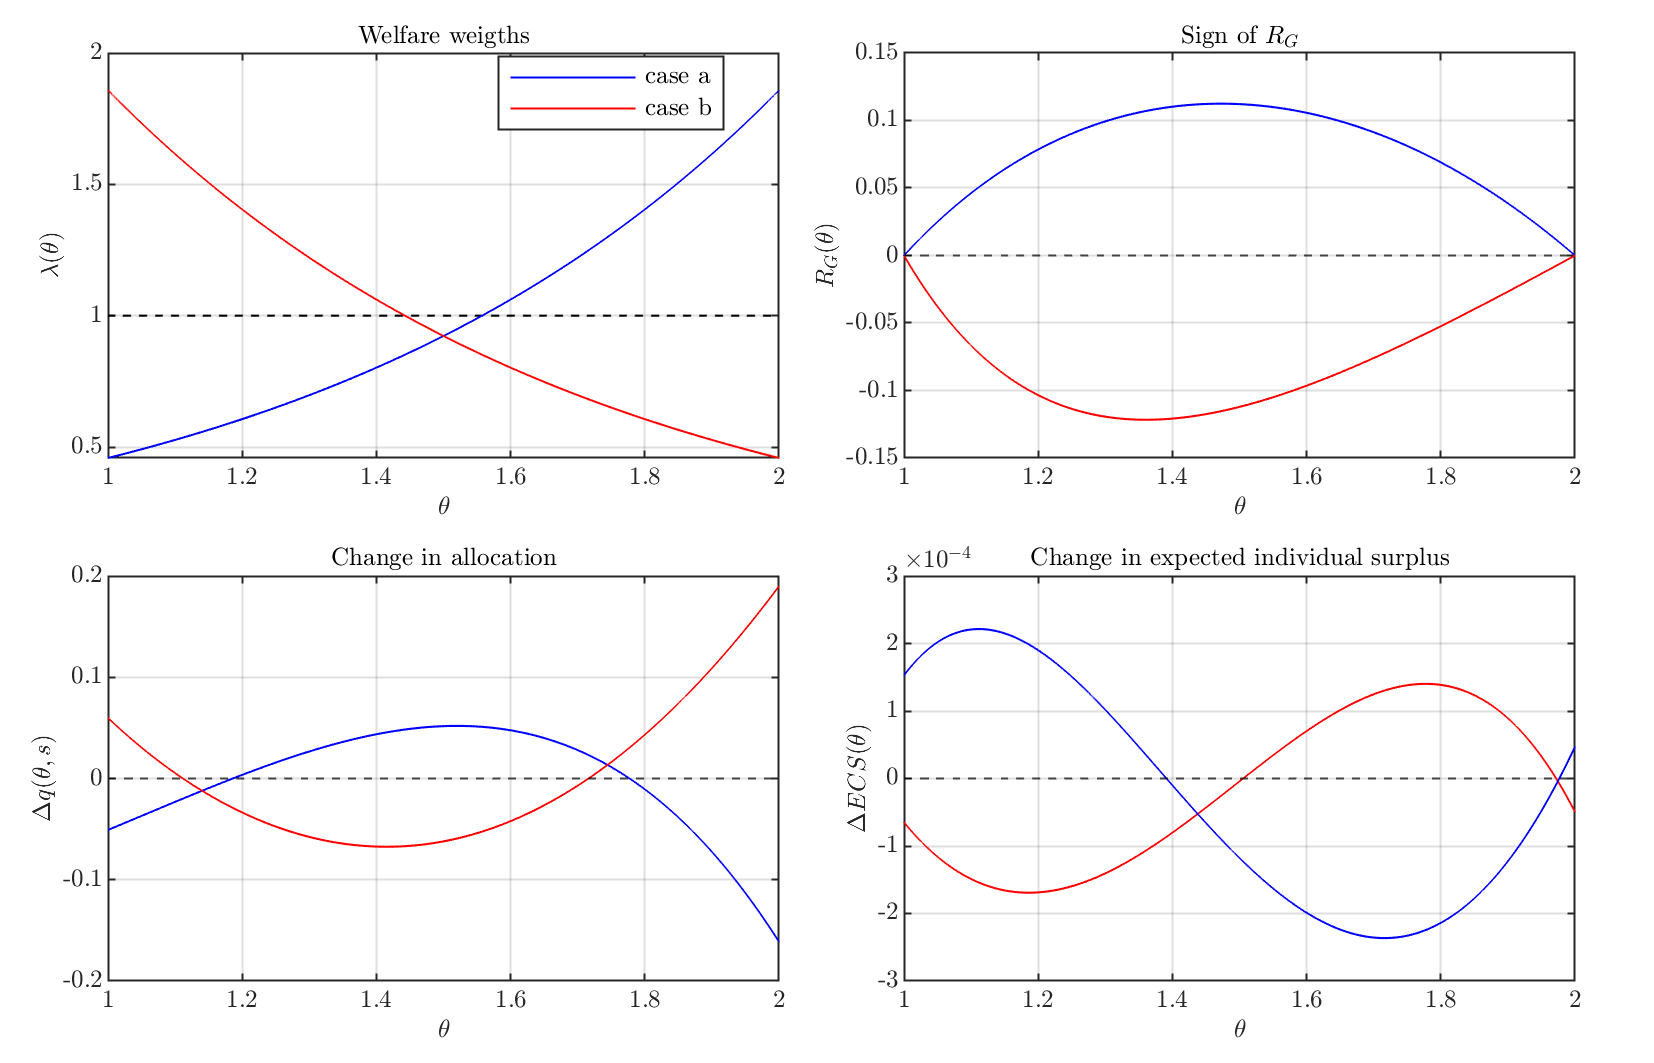
\includegraphics[width=0.8\linewidth]{figure/appendix_withinperturbation.png}
\end{figure}

\end{frame}

%-----------------------------------------------------------%
\begin{frame}{Across-category allocation: setup 1 }
Given within-category value functions $V_i(k_i, I_i)$, the designer solves:
\[ \max_{\{k_i, I_i\}_{i \in N}} \sum_i \mu_i V_i(k_i, I_i) \quad \text{s.t.} \quad \sum_i \mu_i k_i = k, \quad \sum_i \mu_i I_i = I(k), \quad k_i, I_i \geq 0 \]
where $V_i(k_i, I_i) := \max_{q_i(\theta,s)} \E_{(s,i)}[\Gamma_i(\theta)U(q_i(\theta,s),s)] - \tilde\lambda_i I_i$.
\vspace{0.2cm}
\textbf{Envelope theorem applied to $V_i$:}
\begin{columns}
\begin{column}{0.48\textwidth}
\begin{block}{Marginal value of capacity}
\[ \Pi_i(k_i,I_i) := \partial_{k_i} V_i = \E_s[\varepsilon_i(s)\,\mathbf{1}_{\{s \in T_i\}}] \]
Expected shadow value of relaxing the capacity constraint. Equals the expected aggregate marginal utility generated by extra capacity, weighted by $\G_i(\theta)$.
\end{block}
\end{column}
\begin{column}{0.48\textwidth}
\begin{block}{Marginal social cost of revenue}
\[ \partial_{I_i} V_i = -\tilde\lambda_i - \beta_i(k_i, I_i) \]
$\beta_i$ captures the canonical cost of tightening the budget; $\tilde\lambda_i$ captures the additional social cost from redistributive concerns.
\end{block}
\end{column}
\end{columns}

\end{frame}

\begin{frame}{Across-category allocation: setup 2}

\begin{lemma}[Across-category optimality, Lemma outer]
At the optimum: $\Pi_i(k_i^\ast,I_i^\ast) = \zeta_k$ and $\tilde\lambda_i + \beta_i(k_i^\ast,I_i^\ast) = -\zeta_I + \xi_i$ with $\xi_i I_i^\ast = 0$.
\end{lemma}

\vspace{0.2cm}

The designer equalizes scarcity rents across categories and equalizes the effective marginal social cost of revenue across contributing categories.

\vspace{0.2cm}

Using the first-order conditions in the previous Lemma, consider the induced difference in the marginal value of capacity around category \(i\):

\vspace{0.2cm}

\[
\Delta \Pi_i(k_i^\ast,I_i^\ast)
=
\E_{(s,i)}\![
(
\underbrace{u_q(q_i(\theta,s),s)\,\G_i(\theta)\,\Delta q_i(\theta,s)
}_{\text{behavioral effect}}+
\underbrace{u(q_i(\theta,s),s)\,\Delta \G_i(\theta)}_{\text{weight effect}}
)
\mathbf{1}_{\{s\in T_i\}}
].
\]
\end{frame}

%-----------------------------------------------------------%
\begin{frame}{Theorem: capacity ranking 1}
\begin{theorem}[Capacity ranking]
Suppose category $j$ differs from baseline category $i$ only through a marginal perturbation of redistributive preferences. Fix the baseline optimum $(k_i^\ast, I_i^\ast)$. Then, to first order in $\Delta\lambda$:
\[ k_j^\ast > k_i^\ast \iff \E_s\!\left[\varepsilon_i(s)\, \E_i^w\!\left[R_\G \mid s\right]\, \mathbf{1}_{\{s \in T_i\}}\right] > 0 \]
Under CARA, this reduces to $k_j^\ast > k_i^\ast$ iff $\E_i[R_\G(\theta)] > 0$.
\end{theorem}
\vspace{0.2cm}
\textbf{Key implication:} The relevant comparison is \emph{not} which category has the larger average effective weight, but whether category $j$'s advantage is concentrated on types for which category $i$'s effective weight is \emph{low}.

\end{frame}

%-----------------------------------------------------------%
\begin{frame}{Theorem: capacity ranking 2}
\begin{alertblock}{Policy lesson}
Categories should be ranked not by the absolute size of the difference in redistributive preferences, but by the \emph{relative distribution} of their effective social weights across types. Two categories may have the same absolute difference in welfare weights and receive \emph{opposite} capacity rankings.
\end{alertblock}
\vspace{0.2cm}
\textbf{Connection to within-category analysis:} The same object $R_\G(\theta)$ that governed the reallocation of quantities and the surplus effects of preference differences \emph{within} a category now determines which category receives more capacity at the outer optimum.
\end{frame}
%-----------------------------------------------------------%
\begin{frame}{Appendix figure: absolute vs proportional ranking can diverge}

\begin{figure}
    \centering
    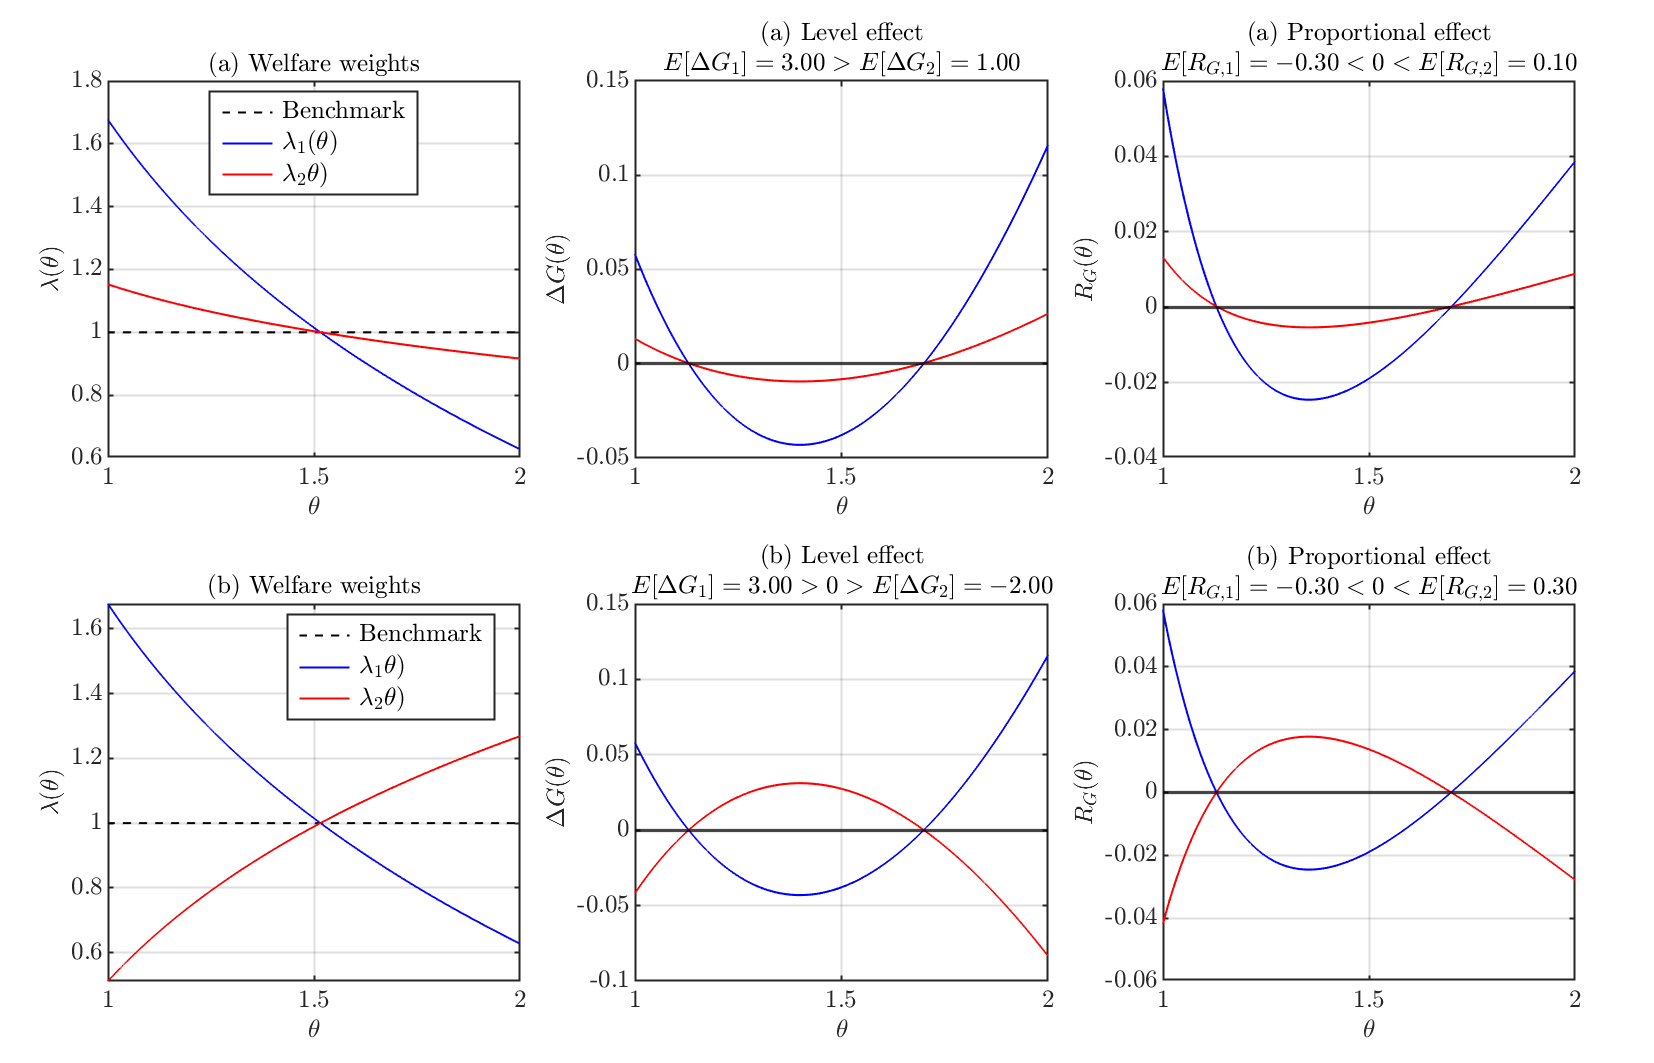
\includegraphics[width=0.8\linewidth]{figure/appendix_two_scenarios_six_panels.png}

\end{figure}


\end{frame}

%-----------------------------------------------------------%
\begin{frame}{Corollary: capacity ordering along an ordered preference path}
\begin{block}{Assumption: Ordered preference path}
For each adjacent pair $(i-1, i)$, there exists a $C^1$ path $\lambda(t,\theta)$ on $[0,1]\times\Theta$ connecting $\lambda_{i-1}(\theta)$ to $\lambda_i(\theta)$, along which for all $t$:
\begin{enumerate}
\item[(i)] Average weight is weakly increasing: $\partial_t \tilde\lambda(t) \geq 0$.
\item[(ii)] Relative tilt is toward higher types: $\partial_t \log\lambda(t,\theta)$ is weakly increasing in $\theta$.
\end{enumerate}
\end{block}
\begin{corollary}[Capacity ordering]
Under the ordered preference path assumption, the equilibrium capacity profile is globally weakly monotone:
\[ k_1^\ast \leq k_2^\ast \leq \cdots \leq k_n^\ast \]
\end{corollary}
\vspace{0.2cm}
\textbf{Why both conditions (i) and (ii) are necessary:}
\begin{itemize}
\item Condition (i) alone (higher average weight) is not sufficient for more capacity.
\item Condition (ii) ensures proportionally stronger weighting of higher types, which enlarges $\G_i(\theta)$ through the IC term $\Lambda_i(\theta)$.
\end{itemize}
\end{frame}

%-----------------------------------------------------------%
\begin{frame}{Appendix figure: capacity ordering across 50 categories}

\begin{figure}
    \centering
    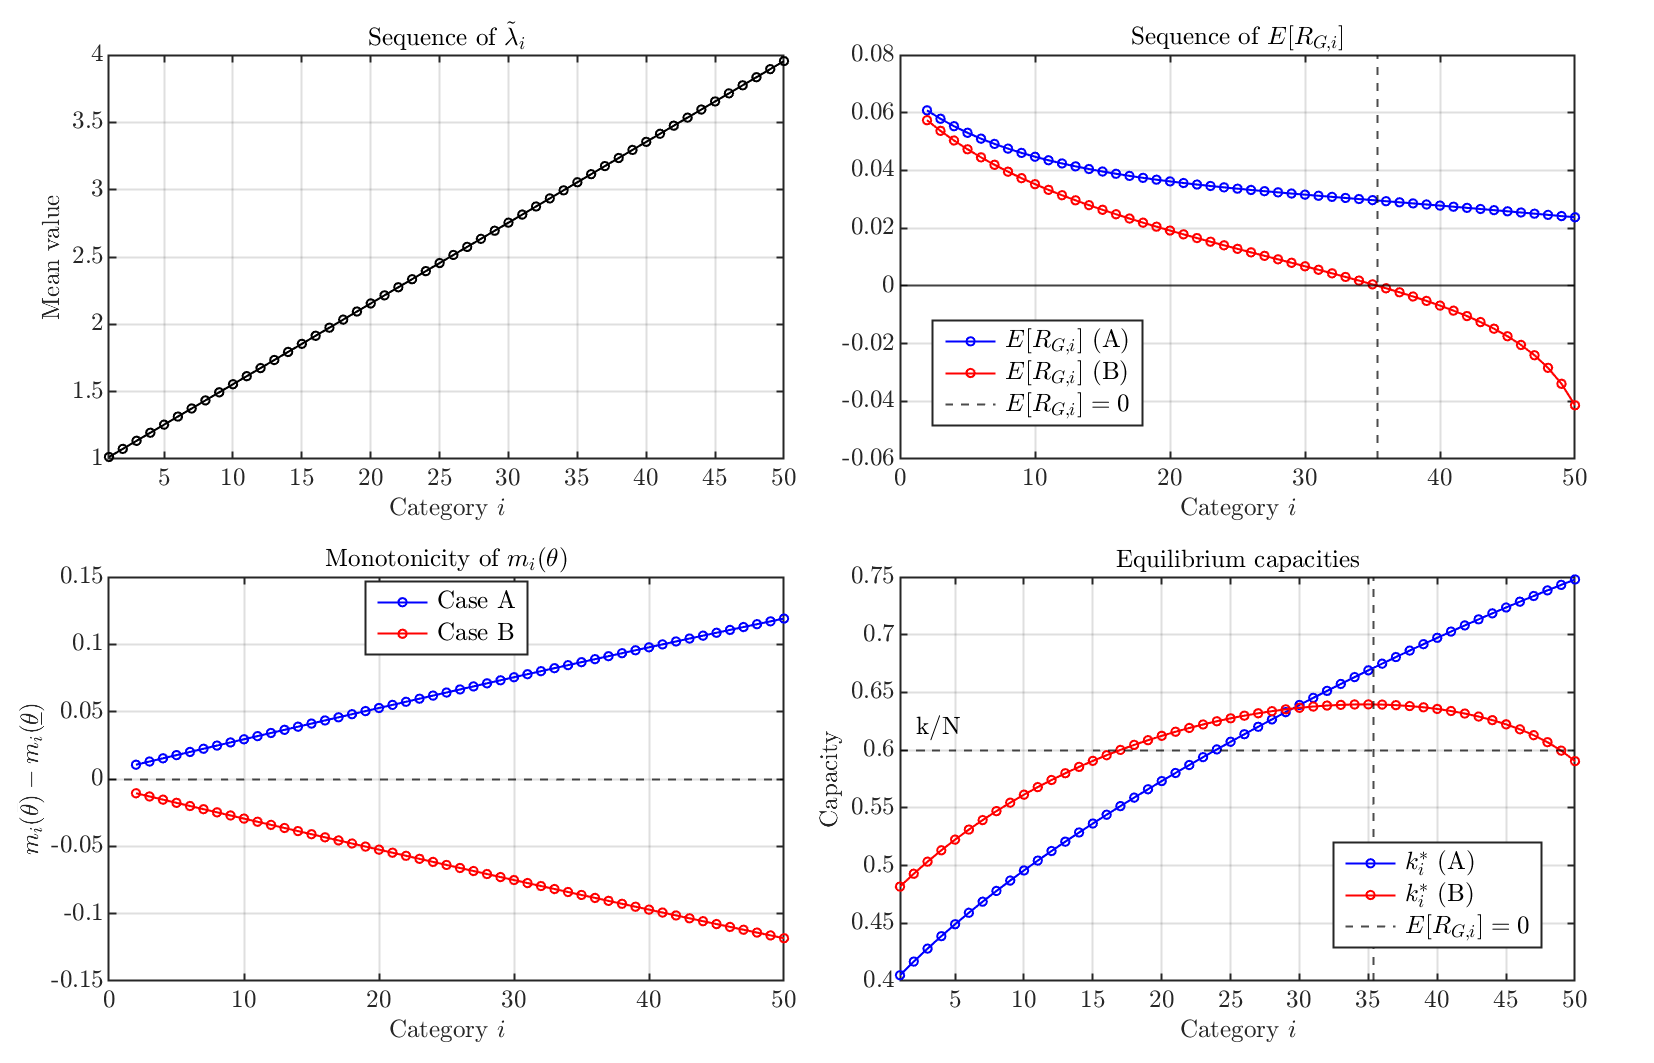
\includegraphics[width=0.8\linewidth]{figure/appendix_N_categories_six_panels.png}

\end{figure}


\end{frame}

%-----------------------------------------------------------%
\begin{frame}{Proposition: revenue ordering}
\begin{theorem}[Revenue ordering]
Define $N^+ = \{i : \beta_i^\ast > 0\}$ (contributing) and $N^0 = \{i : \beta_i^\ast = 0\}$ (non-contributing).

\textbf{Extensive margin:} At any equilibrium, $\max_{i \in N^+} \tilde\lambda_i < \min_{i \in N^0} \tilde\lambda_i$. The contributor/non-contributor split is governed solely by \emph{average welfare weights}, regardless of within-type structure.

\textbf{Intensive margin:} For $i, j \in N^+$ with $\Delta k = k_j^\ast - k_i^\ast > 0$:
\[ I_j^\ast < I_i^\ast \iff -\underbrace{\left(\Delta k \frac{\partial \beta_i}{\partial k_i} + \Delta_\lambda \beta_i\right)}_{\text{revenue effect}} < \underbrace{\Delta\tilde\lambda}_{\text{preference effect}} \]
\end{theorem}
\vspace{0.1cm}
\textbf{Three rankings need not coincide:}
\begin{itemize}
\item Capacity ranking: governed by $\E_i[R_\G(\theta)]$ (proportional).
\item Extensive revenue margin: governed by $\tilde\lambda_i$ (average welfare weights alone).
\item Intensive revenue margin: governed by the interaction of \emph{both} sorting margins.
\end{itemize}
\end{frame}

%-----------------------------------------------------------%
\begin{frame}{Optimal investment: the incomplete-information peak-load rule}
\begin{lemma}[Optimal investment]
The problem $\max_{k \geq 0} W(k)$ admits a unique interior solution $k^\ast > 0$ satisfying:
\[ I'(k^\ast) = \frac{1}{\mu^+ \tilde\lambda^\ast} \sum_{i \in N^+} \mu_i\, \Pi_i(k_i^\ast,I_i^\ast) = \frac{1}{\mu^+} \sum_{i \in N^+} \mu_i\, \E_{(s,i)}\!\left[u(q_i,s)\,\frac{\G_i(\theta)}{\tilde\lambda^\ast}\,\mathbf{1}_{\{s \in T_i\}}\right] \]
where $\mu^+ = \sum_{i \in N^+} \mu_i$ and $\tilde\lambda^\ast = -\zeta_I > 0$ is the equilibrium marginal cost of funds. Moreover, $\max_{i \in N^+} \tilde\lambda_i < \tilde\lambda^\ast \leq \min_{i \in N^0} \tilde\lambda_i$.
\end{lemma}
\vspace{0.2cm}
\textbf{Comparison with classical peak-load rule:} Under complete information with redistribution, there are no IC rents so $J_i(\theta) = \theta$ and $\Lambda_i(\theta) = 0$, which gives $\G_i(\theta)/\tilde\lambda^\ast \to \theta$, recovering the standard rule.
\vspace{0.2cm}
\begin{alertblock}{Key departure under redistributive preferences}
Under utilitarian preferences, IC rents are welfare-neutral (pure transfers in the social objective), so complete- and incomplete-information investment rules \emph{coincide} at the optimum. Under redistributive preferences, IC rents are no longer welfare-neutral, and the informational wedge \emph{persists even at $k^\ast$}.
\end{alertblock}
\end{frame}

%-----------------------------------------------------------%
\begin{frame}{Appendix figure: welfare under complete vs incomplete information}

\begin{figure}
    \centering
    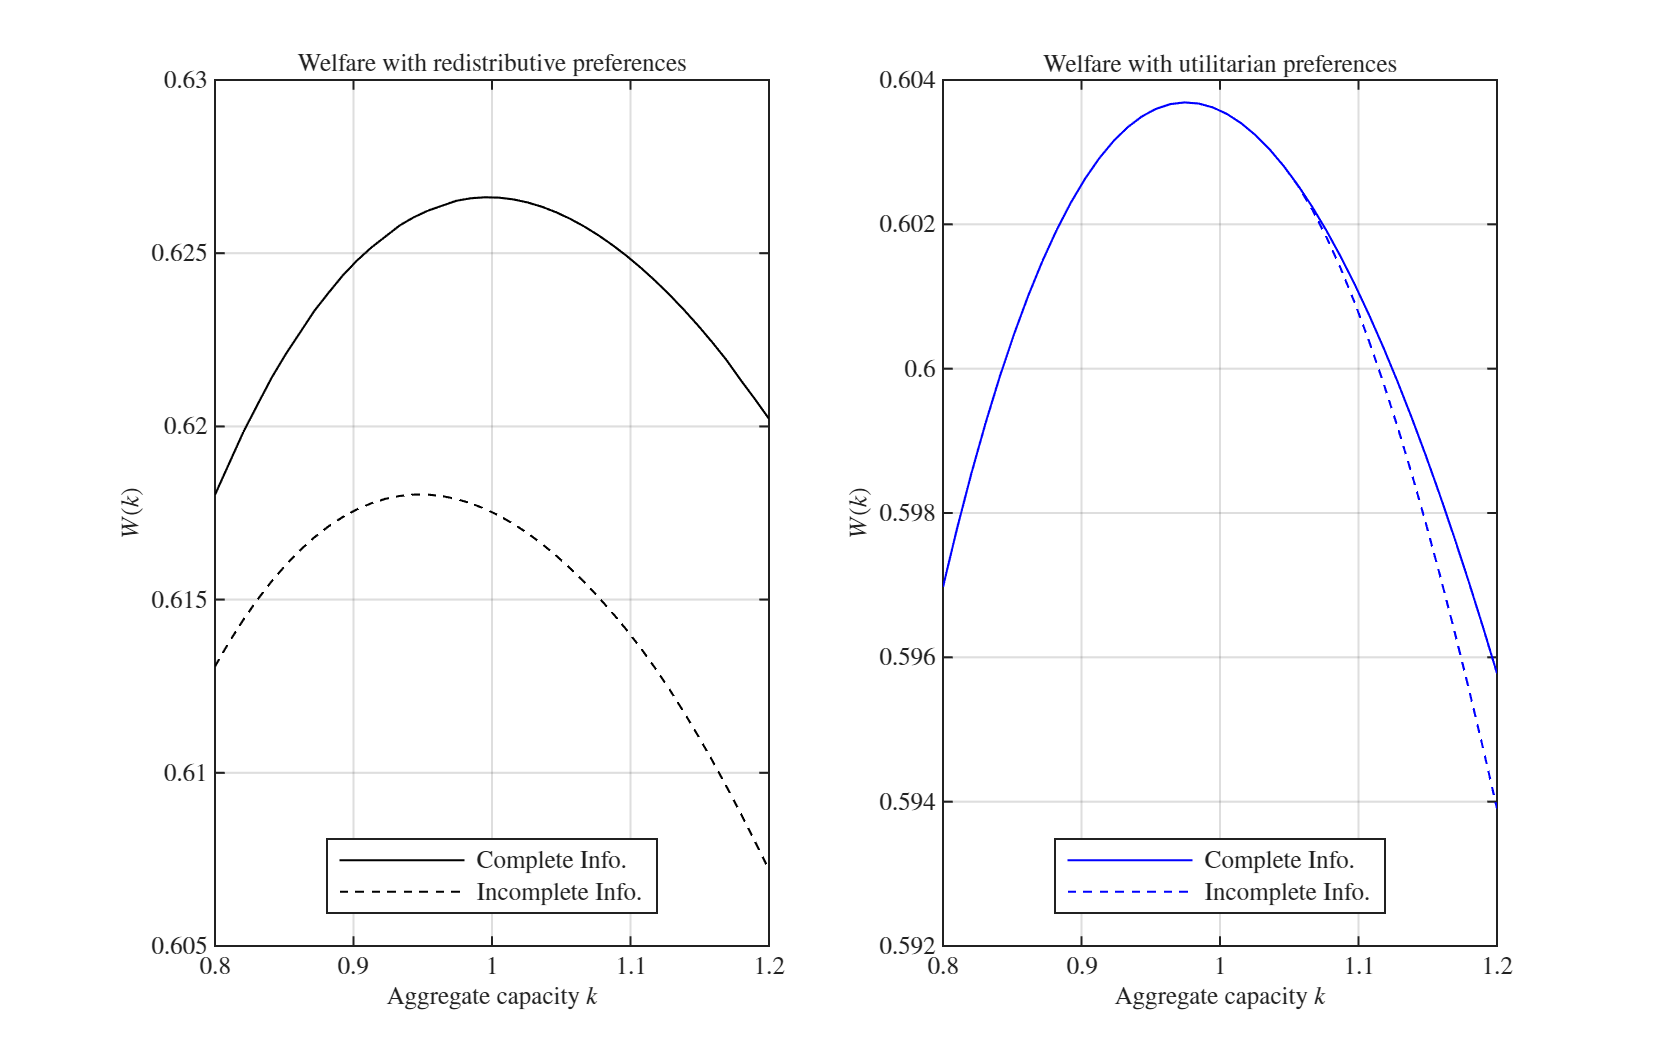
\includegraphics[width=0.8\linewidth]{figure/appendix_OptimalFBSB.png}
\end{figure}

\end{frame}

%-----------------------------------------------------------%
\begin{frame}{Proposition: investment response to redistributive preference perturbations}
\begin{proposition}[Investment response]
Under CARA, a marginal mean-preserving perturbation of $\lambda_i(\theta)$ induces:
\[ W''(k^\ast)\,\Delta k^\ast = -\underbrace{\sum_i \mu_i\,\Pi_i\,\E_i[R_{\G,i}]}_{\text{average effect}} + \underbrace{I'(k^\ast)\,\Delta\tilde\lambda^\ast}_{\text{sorting effect}} \]
where $W''(k^\ast) < 0$ and
\[ \Delta\tilde\lambda^\ast = -\frac{\sum_{i \in N^+} \mu_i\,\overline\varepsilon_i\,\Cov_i(R_{\theta,i}, R_{\G,i})}{\sum_{i \in N^+} \mu_i\,\overline\varepsilon_i\,\Var_i(R_{\theta,i})} \]
\end{proposition}
\vspace{0.2cm}
\textbf{Two channels:}
\begin{enumerate}
\item \textbf{Average effect:} A preference perturbation changes the marginal value of capacity $\Pi_i$ across categories. Under an ordered path with $\E_i[R_{\G,i}] > 0$, this term pushes toward \emph{higher} investment.
\item \textbf{Sorting effect:} The perturbation changes $\tilde\lambda^\ast$, the equilibrium marginal cost of funds. Its sign is governed by the covariance between $R_{\theta,i}$ and $R_{\G,i}$, connecting back to the within-category sorting analysis.
\end{enumerate}
\vspace{0.1cm}
\textbf{Policy:} For optimal investment to increase, the preference perturbation must raise scarcity rents on average \emph{and} align with the distribution of marginal virtual utility across types within contributing categories.
\end{frame}

%-----------------------------------------------------------%
\begin{frame}{Appendix figure: optimal investment level under preference perturbations}
\begin{figure}
    \centering
    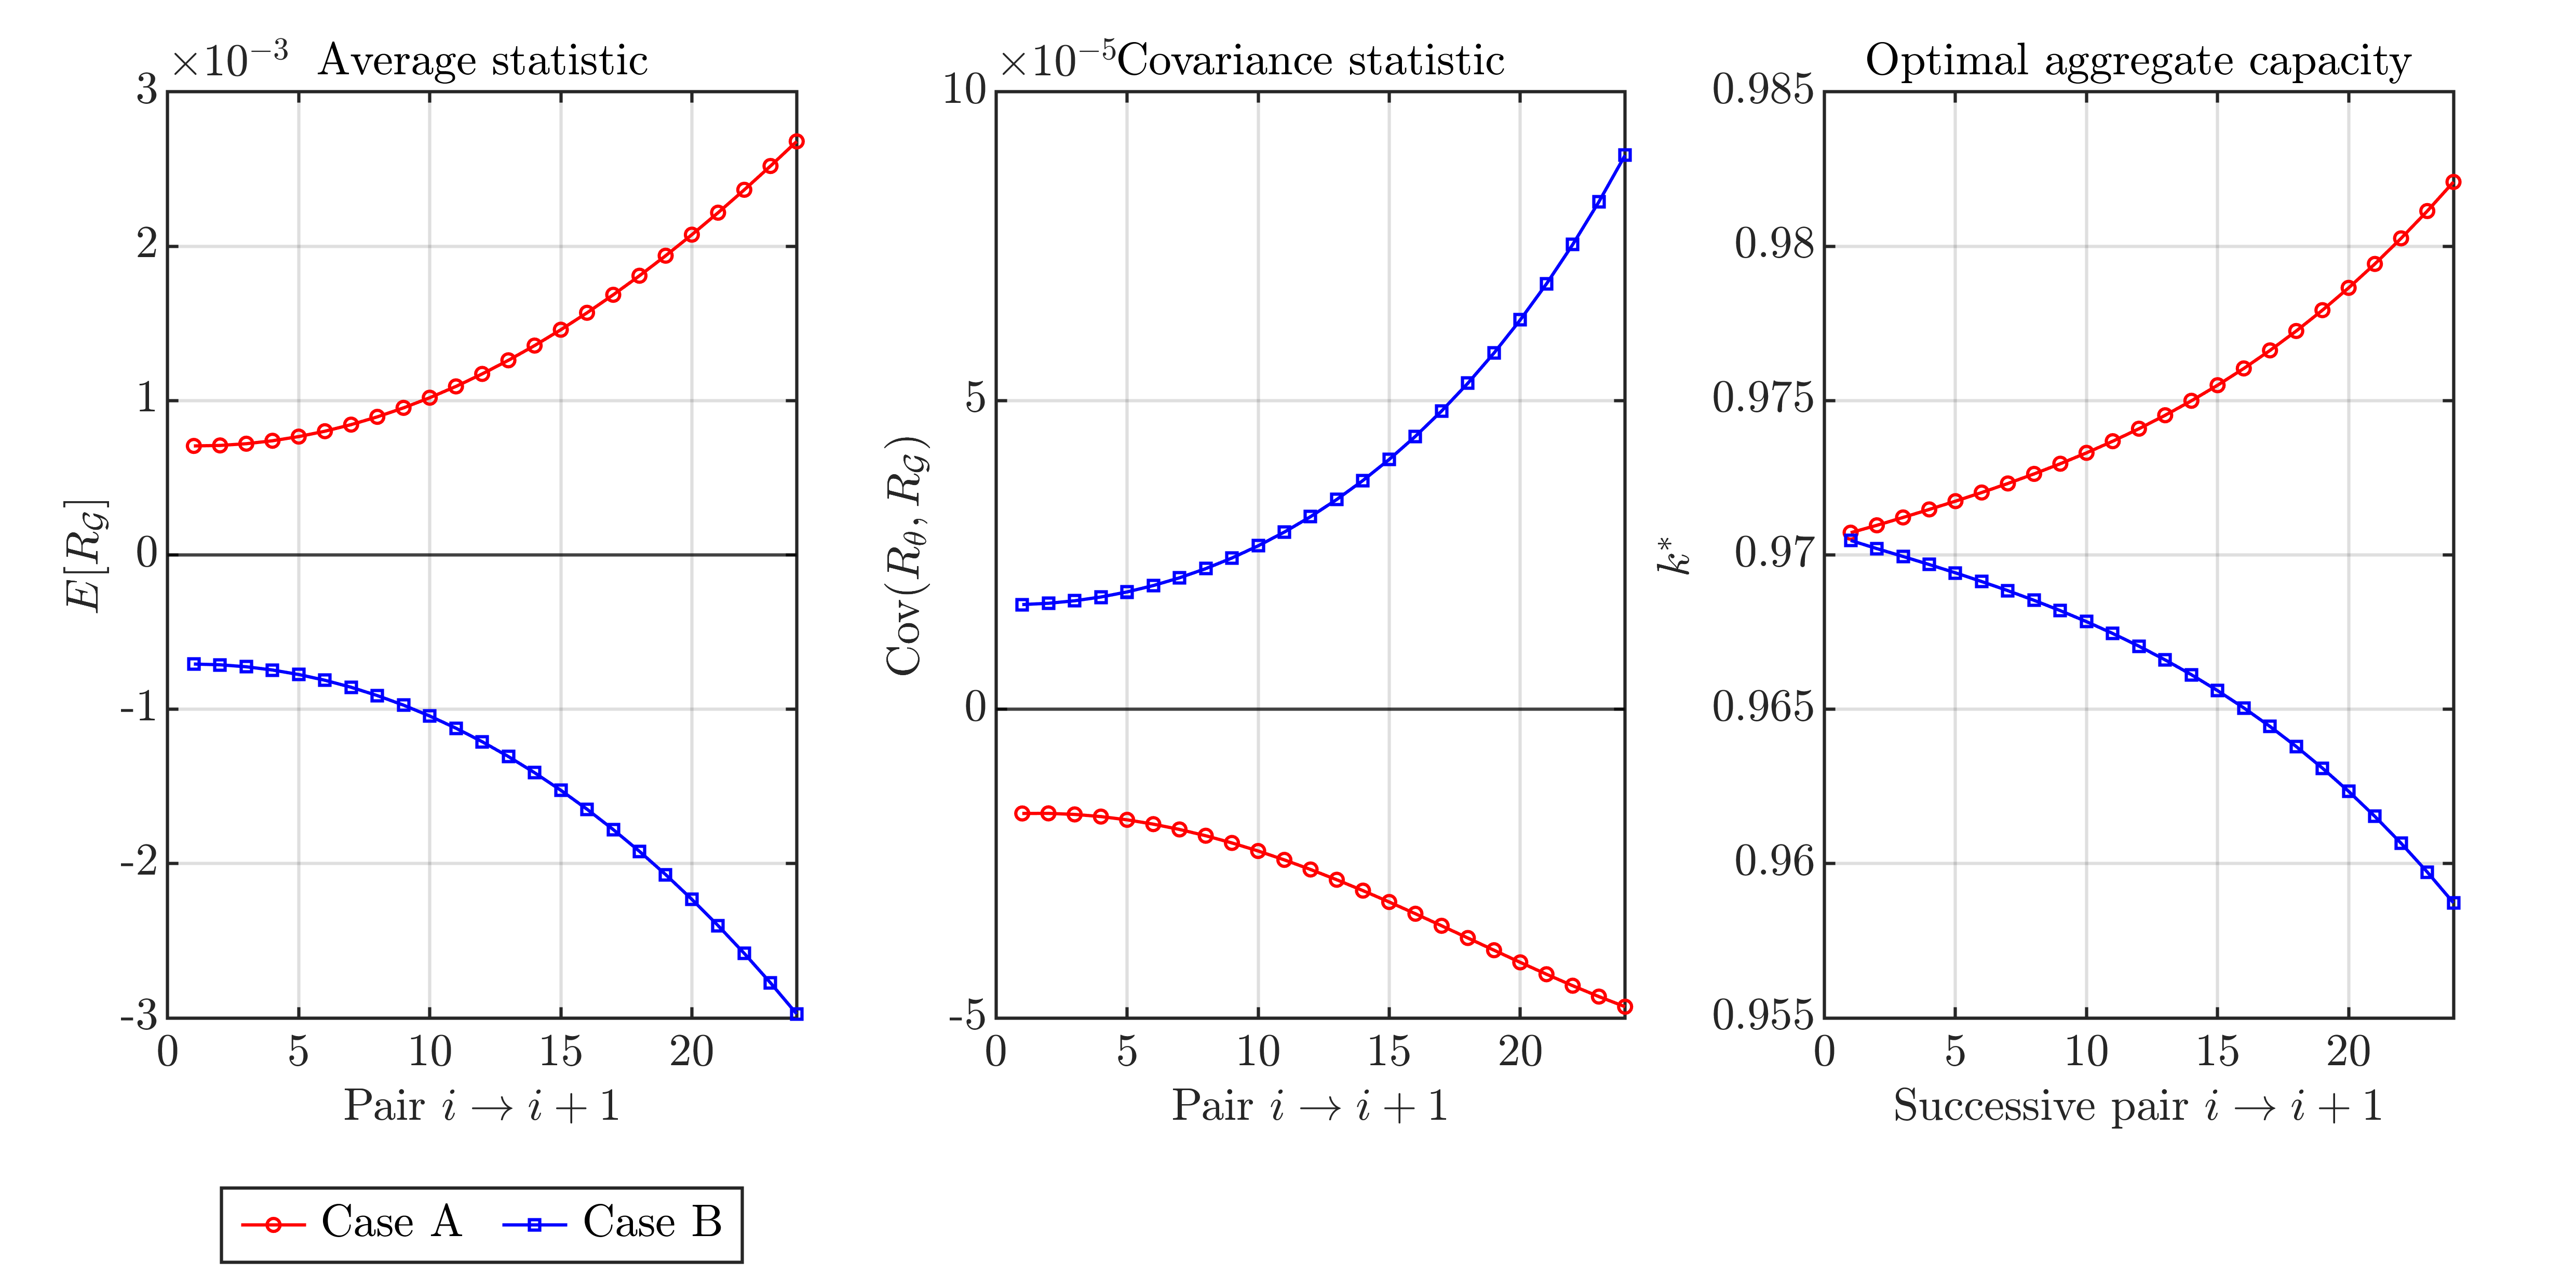
\includegraphics[width=0.8\linewidth]{figure/appendix_exampleoptimallevel.png}
\end{figure}

\end{frame}


%-----------------------------------------------------------%
\begin{frame}{Redistributive incidence of a global capacity expansion}
The full surplus effect decomposes as:
\[ \frac{d\,\E CS_i(\theta)}{dk} = \underbrace{\frac{\partial \E CS_i(\theta)}{\partial k_i}}_{\text{within-category incidence}} \cdot \underbrace{\frac{dk_i^\ast}{dk}}_{\text{cross-category response}} \]

\textbf{What governs $dk_i^\ast/dk$?} From Lemma dkidk, category $i$ receives more of the expansion whenever its \emph{marginal revenue exceeds its marginal cost}:
\[ \sign\!(\underbrace{\E_{(s,i)}^w[uJ \mid s]}_{\text{category-level marginal revenue}} - \underbrace{I'(k^\ast)}_{\text{marginal cost}}) \cdot \sign\! (\quad \sum_j \mu_j\,\Omega_j^{-1}\!(\E_{(s,j)}^w[uJ \mid s] - I'(k^\ast) \quad ) \]
The \textbf{first term} is category-specific. The \textbf{second term} is aggregate — it governs the direction of reallocation across all categories simultaneously. \textbf{Both signs together} determine who gains capacity.
\end{frame}


%-----------------------------------------------------------%
\begin{frame}{Redistributive incidence of a global capacity expansion}
\textbf{Two complications make the final incidence non-trivial:}
\begin{itemize}
\item The sign of $\E_{(s,i)}^w[uJ\mid s]$ is itself \emph{level-dependent}: from Lemma SC-dir, it is single-crossing in $k_i$, so whether category $i$ is above or below its marginal cost threshold depends on where it currently sits on the capacity schedule.
\item The aggregate sign can generate \textbf{convergence} (expansion flows toward low-capacity categories) or \textbf{divergence} (expansion flows toward high-capacity categories), independently of individual category preferences.
\end{itemize}
\end{frame}

%-----------------------------------------------------------%

%-----------------------------------------------------------%
\begin{frame}{Figure: convergence vs divergence of a global capacity expansion}
\begin{figure}
\centering
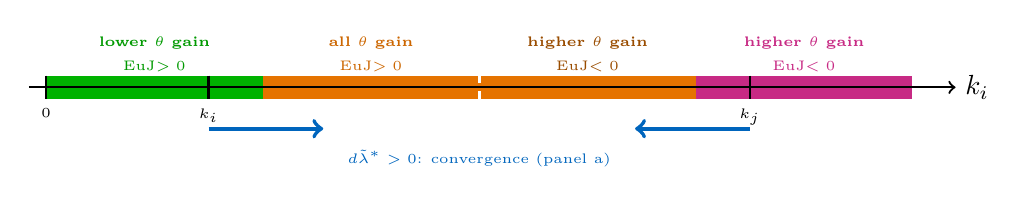
\begin{tikzpicture}[x=1.1cm, y=0.75cm]
\fill[green!70!black]   (0,-0.2) rectangle (2.5,0.2);
\fill[orange!90!black]  (2.5,-0.2) rectangle (5.0,0.2);
\fill[orange!90!black]  (5.0,-0.2) rectangle (7.5,0.2);
\fill[magenta!80!black] (7.5,-0.2) rectangle (10.0,0.2);
\draw[white, dashed, line width=1pt] (5.0,-0.2) -- (5.0,0.2);
\node[font=\tiny\bfseries, green!60!black]   at (1.25,0.75) {lower $\theta$ gain};
\node[font=\tiny\bfseries, orange!80!black]  at (3.75,0.75) {all $\theta$ gain};
\node[font=\tiny\bfseries, orange!60!black]  at (6.25,0.75) {higher $\theta$ gain};
\node[font=\tiny\bfseries, magenta!80!black] at (8.75,0.75) {higher $\theta$ gain};
\node[font=\tiny, green!60!black]   at (1.25,0.35) {EuJ$>0$};
\node[font=\tiny, orange!80!black]  at (3.75,0.35) {EuJ$>0$};
\node[font=\tiny, orange!60!black]  at (6.25,0.35) {EuJ$<0$};
\node[font=\tiny, magenta!80!black] at (8.75,0.35) {EuJ$<0$};
\draw[->, thick] (-0.2,0) -- (10.5,0);
\node[right] at (10.5,0) {$k_i$};
\foreach \x/\lbl in {0/$0$, 1.875/$k_i$, 8.125/$k_j$}{
\draw[thick] (\x,0.2) -- (\x,-0.2);
\node[below, font=\tiny] at (\x,-0.2) {\lbl};
}
\draw[->, line width=1.5pt, aaltoBlue] (1.875,-0.7) -- (3.2,-0.7);
\draw[->, line width=1.5pt, aaltoBlue] (8.125,-0.7) -- (6.8,-0.7);
\node[font=\tiny, aaltoBlue] at (5.0,-1.2) {$d\tilde\lambda^\ast > 0$: convergence (panel a)};
\end{tikzpicture}
\end{figure}
\vspace{0.1cm}
\textbf{Panel (a):} $d\tilde\lambda^\ast > 0$: the expansion reallocates capacity toward the low-capacity category $i$ and away from the high-capacity category $j$, compressing cross-category heterogeneity.

\textbf{Panel (b) [not shown]:} $d\tilde\lambda^\ast < 0$: the directions of the arrows reverse — the expansion pushes the two categories further apart, deepening redistribution divergence.

\textbf{Under Figure (b) of implementation geometry} (where EuJ crosses from $-$ to $+$), the directions of the arrows are reversed at each capacity level.
\end{frame}

%-----------------------------------------------------------%
\begin{frame}{Complete-information benchmark: contrast with private information}
\begin{block}{Complete-information optimal allocation (Proposition FBalloc)}
On-peak, the allocation satisfies:
\begin{itemize}
\item \textbf{Contributing types} ($\lambda_i(\theta) \leq \lambda^\ast$): $u(q_i^\ast,s)\cdot\beta\theta = \varepsilon(s)$. Full surplus extraction, common scarcity price $\varepsilon(s)/\beta$.
\item \textbf{Non-contributing types} ($\lambda_i(\theta) > \lambda^\ast$): $u(q_i^\ast,s)\cdot\lambda_i(\theta)\theta = \varepsilon(s)$. Zero net transfer, type-specific on-peak price $\varepsilon(s)/\lambda_i(\theta)$.
\end{itemize}
\end{block}
\vspace{0.2cm}
\textbf{Two features that disappear under private information:}
\begin{enumerate}
\item \textbf{Sharp partition.} Under complete information, redistribution operates through a clean contributor/non-contributor split at the cutoff type $\lambda_i(\theta) = \lambda^\ast$. Under incomplete information, IC links all types through the rent schedule — revenue extraction becomes category-based and distorts the whole within-category allocation.
\item \textbf{Separability.} Under complete information, redistribution and revenue extraction are largely separable. Under incomplete information, they conflict: changing one type's allocation affects all higher types' informational rents.
\end{enumerate}
\vspace{0.1cm}
$\Rightarrow$ Under complete information, a uniform spot price \emph{fails} to implement the first best (except among contributing types). Under incomplete information, it fails even more severely.
\end{frame}

%-----------------------------------------------------------%
\begin{frame}{Summary of results}
\begin{table}
\small
\begin{tabular}{lll}
\toprule
\textbf{Question} & \textbf{Governing object} & \textbf{Key finding} \\
\midrule
Who benefits from $\uparrow k_i$? & $\E_{(s,i)}^w[uJ \mid s]$ (EuJ) and $R_\theta$ & Non-monotone; sign + regime \\
& & determines winners/losers \\
\midrule
How does $\uparrow \lambda_i$ reshape & $R_\G(\theta) = \Delta\G_i/\G_i$ & Non-monotone; alternating \\
the allocation? & revenue $\Cov_i(R_\theta, R_\G)$ & winner-loser pattern \\
\midrule
Capacity ranking & $\E_i[R_\G(\theta)]$ & Proportional, not absolute \\
across categories & & differences \\
\midrule
Revenue: who contributes? & $\tilde\lambda_i$ (average weight) & Clean separation: $N^+$ vs $N^0$ \\
Revenue: how much? & Both sorting margins & Non-trivial interaction \\
\midrule
Optimal investment rule & $\G_i(\theta)/\tilde\lambda^\ast$ & IC distortion persists at $k^\ast$ \\
& & (unlike utilitarian case) \\
\midrule
Global expansion incidence & $\E_{(s,i)}^w[uJ \mid s]$ vs $I'(k)$ & Convergence vs divergence \\
\bottomrule
\end{tabular}
\end{table}
\end{frame}

%%%%%%%%%%%%%%%%%%%%%%%%%%%%%%%%%%%%%%%%%%%%%%%%%%%%%%%%%%%%%

\begin{frame}{Implementation: nonlinear tariff and block pricing}
    
\begin{figure}
    \centering
    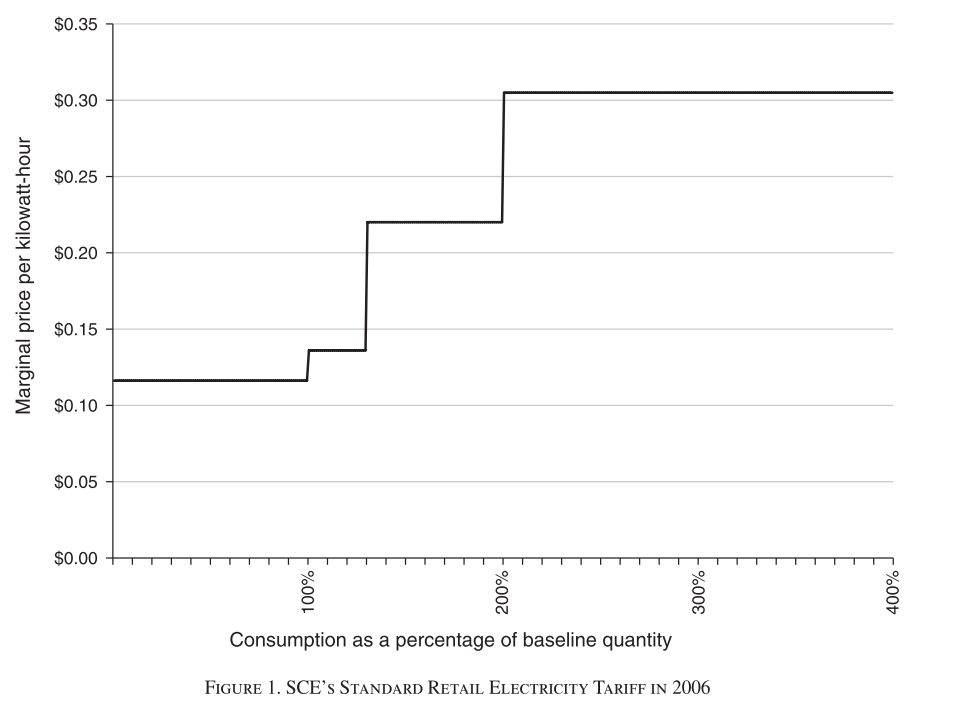
\includegraphics[width=0.7\linewidth]{figure/borenstein.png}
\end{figure}

\end{frame}

%-----------------------------------------------------------%
\begin{frame}{Implementation: nonlinear tariff and block-tariff approximation}
\textbf{Implementing nonlinear tariff.} The optimal mechanism is implemented by a state-contingent tariff under which, after observing $s$, the consumer solves $\max_{q \geq 0}\, \theta U(q,s) - \tau_i(q,s)$. The tariff takes the form:
\[ \tau_i(q,s) = -\E\underline{CS}_i + \int_0^q p_i(x,s)\,dx \]
where $-\E\underline{CS}_i$ is a fixed rebate and the marginal price schedule is:
\[ p_i(q,s) = \theta_i(q,s)\,u(q,s) = \theta \cdot \frac{\varepsilon_i(s)}{\mathcal{G}_i(\theta)}, \qquad s \in T_i \]
\textbf{Block-tariff approximation.} For a partition $0 = q_{i,0} < q_{i,1} < \cdots < q_{i,B}$, the tariff on is:

\[
\tau_i^{BT}(q,s)
=
-\E\underline{CS}_i
+
\sum_{b=1}^B
\pi_{i,b}(s)
\left(\min\left\{q,q_{i,b}\right\}-q_{i,b-1}\right)_+.
\]

where 

\[
\pi_{i,b}(s)
:=
\frac{1}{q_{i,b}-q_{i,b-1}}
\int_{q_{i,b-1}}^{q_{i,b}} p_i(x,s)\,dx.
\]

\end{frame}
%%%%%%%%%%%%%%%%%%%%%%%%%%%%%%%%%%%%%%%%%%%%%%%%%%%%%%%%%%%%%

\begin{frame}{Single category: spot vs. BT}
    
\begin{figure}
    \centering
    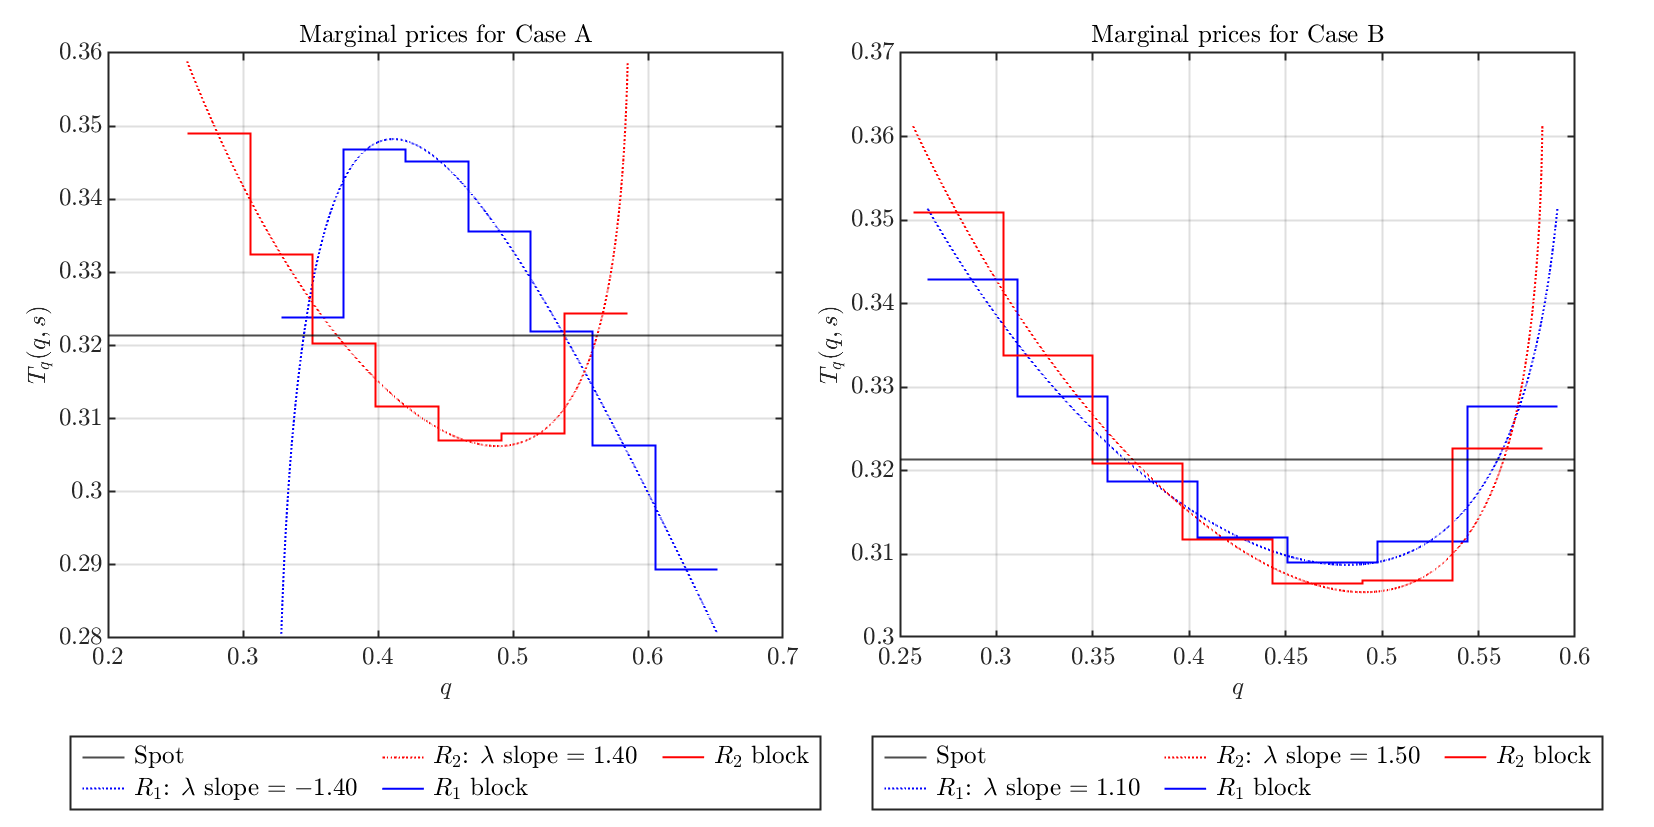
\includegraphics[width=0.9\linewidth]{figure/ImplementationCRRA_decomp.png}
\end{figure}

\end{frame}


%%%%%%%%%%%%%%%%%%%%%%%%%%%%%%%%%%%%%%%%%%%%%%%%%%%%%%%%%%%%%

\begin{frame}{Single category: spot vs. BT}
    
\begin{figure}
    \centering
    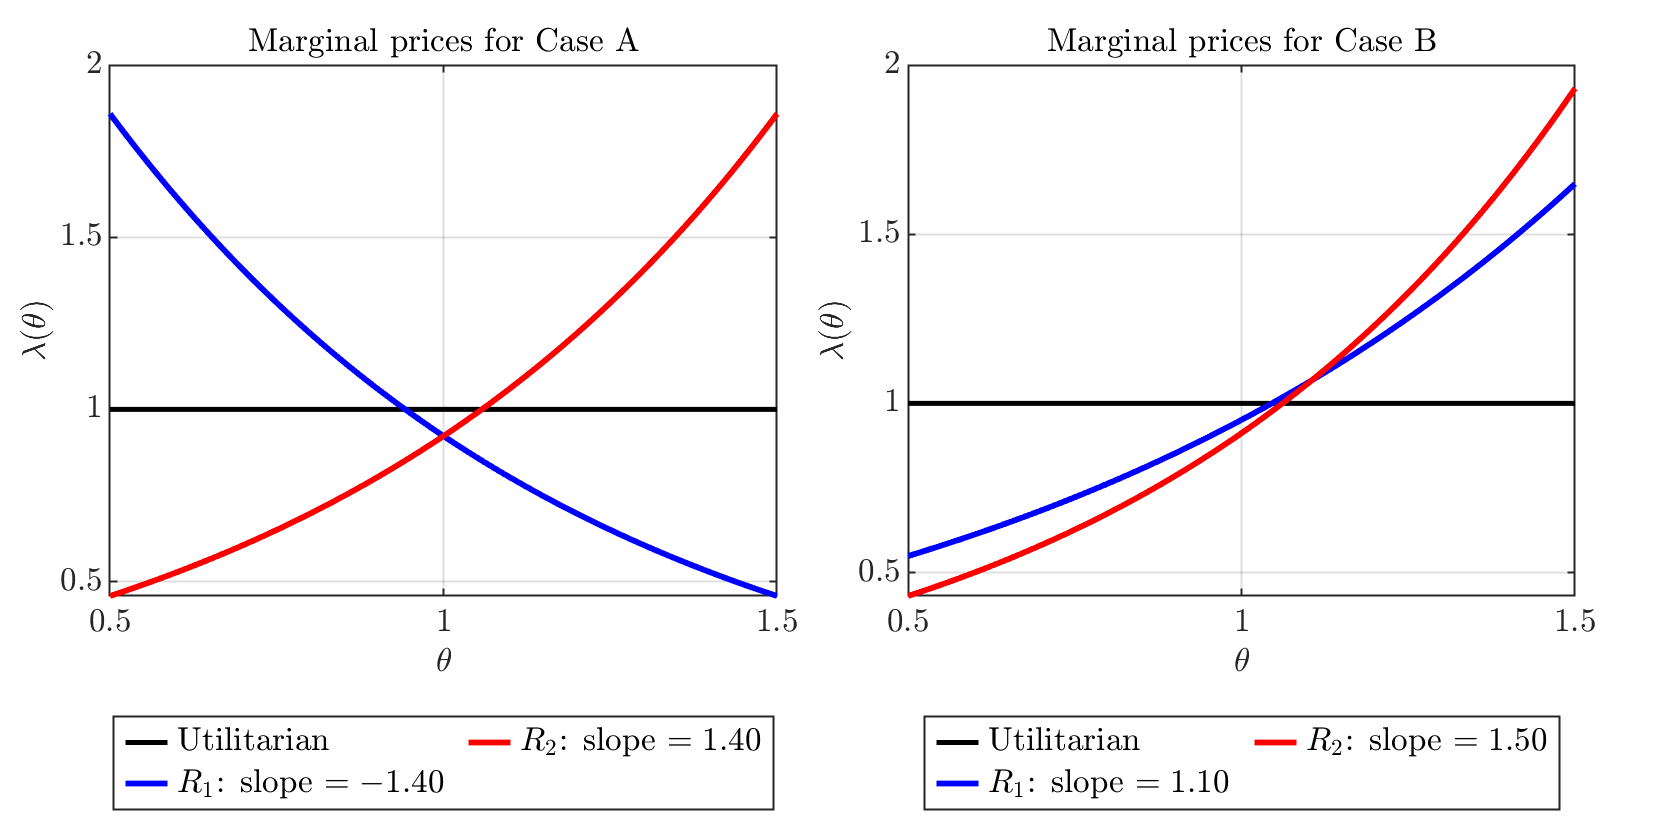
\includegraphics[width=0.9\linewidth]{figure/ImplementationCRRA_lambda.png}
\end{figure}

\end{frame}

%%%%%%%%%%%%%%%%%%%%%%%%%%%%%%%%%%%%%%%%%%%%%%%%%%%%%%%%%%%%%

\begin{frame}{Across category: spot vs. no tag vs optimal}
    
\begin{figure}
    \centering
    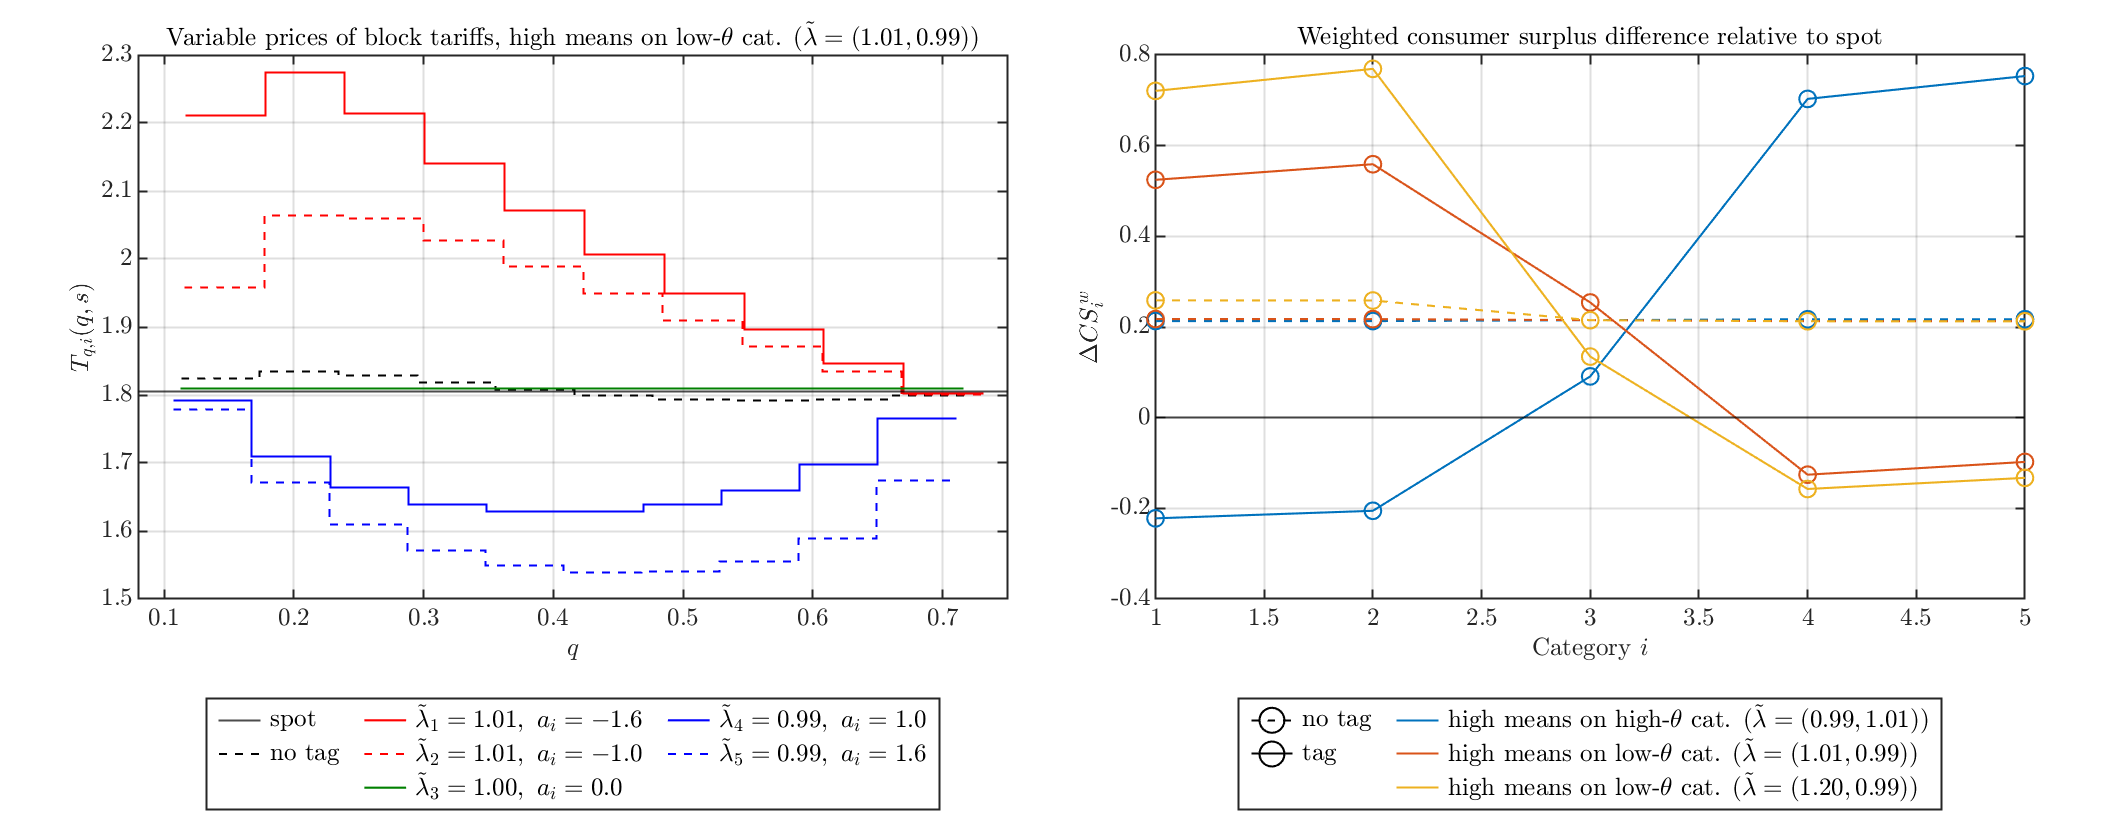
\includegraphics[width=0.9\linewidth]{figure/ImplementationCRRA_Combo_Menu2_CSAll.png}
\end{figure}

\end{frame}

%%%%%%%%%%%%%%%%%%%%%%%%%%%%%%%%%%%%%%%%%%%%%%%%%%%%%%%%%%%%%

\begin{frame}{Across category: spot vs. no tag vs optimal}
    
\begin{figure}
    \centering
    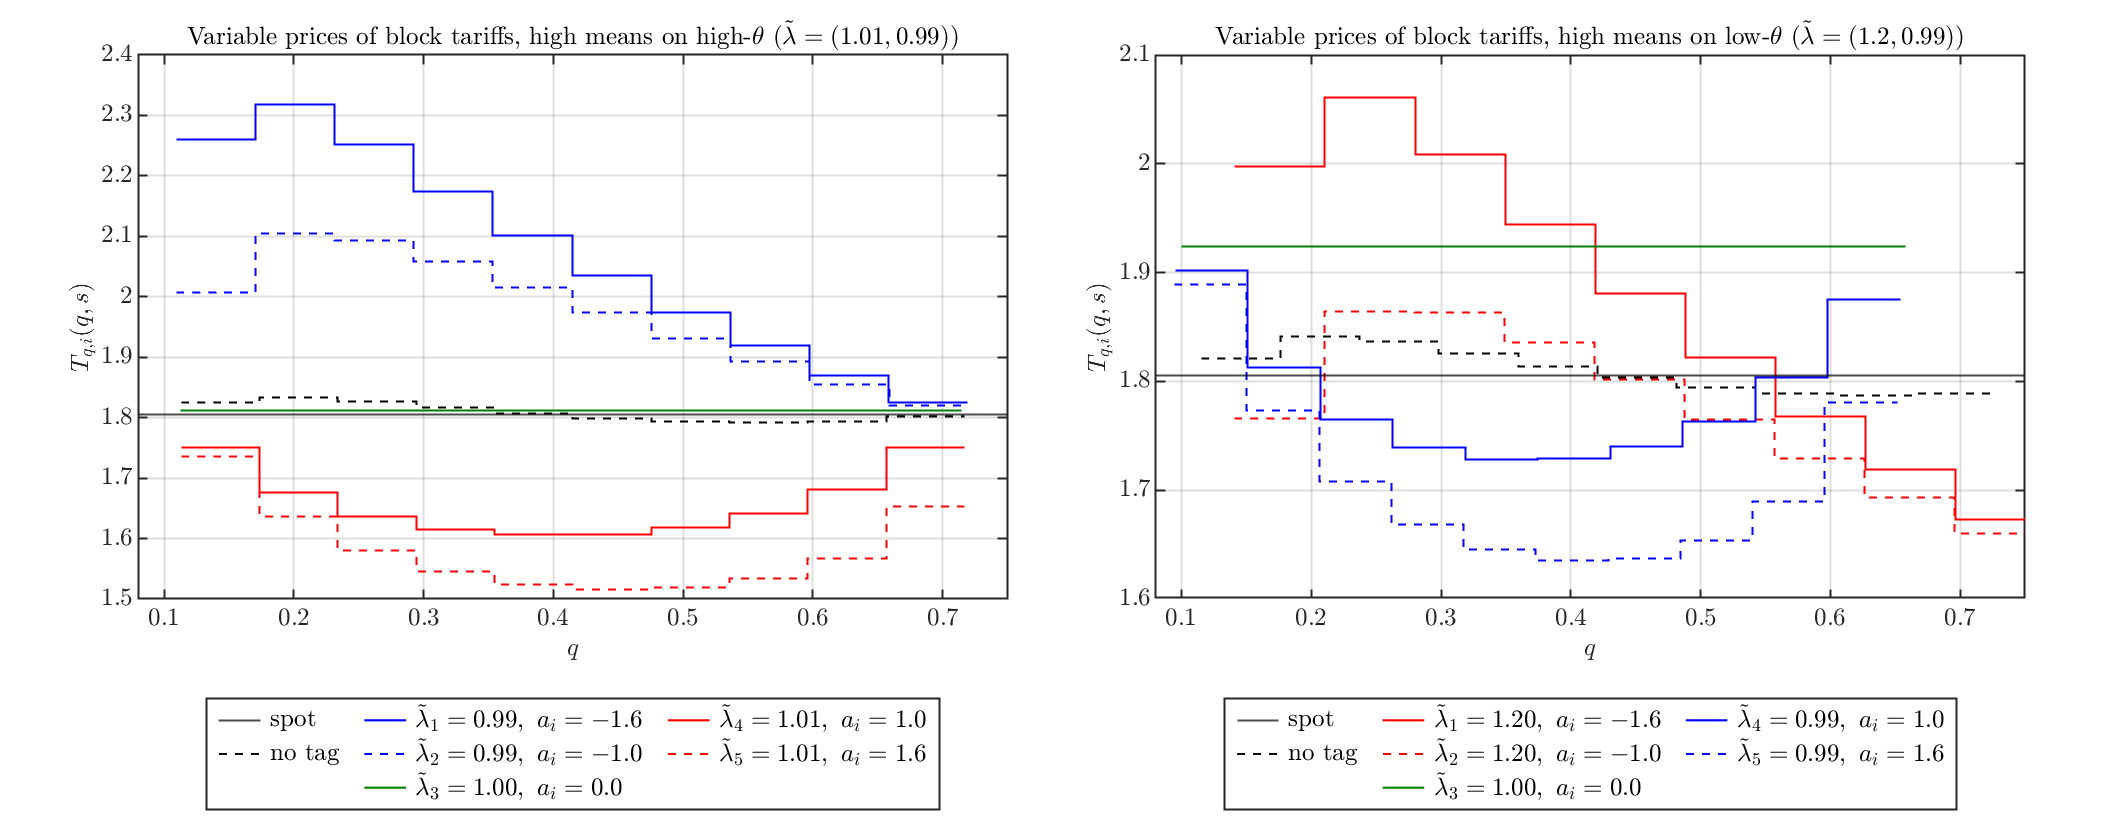
\includegraphics[width=0.9\linewidth]{figure/ImplementationCRRA_Combo_Menu1_Menu3.png}
\end{figure}
\end{frame}
%%%%%%%%%%%%%%%%%%%%%%%%%%%%%%%%%%%%%%%%%%%%%%%%%%%%%%%%%%%%%

\begin{frame}{Across category: spot vs. no tag vs optimal}
    
\begin{figure}
    \centering
    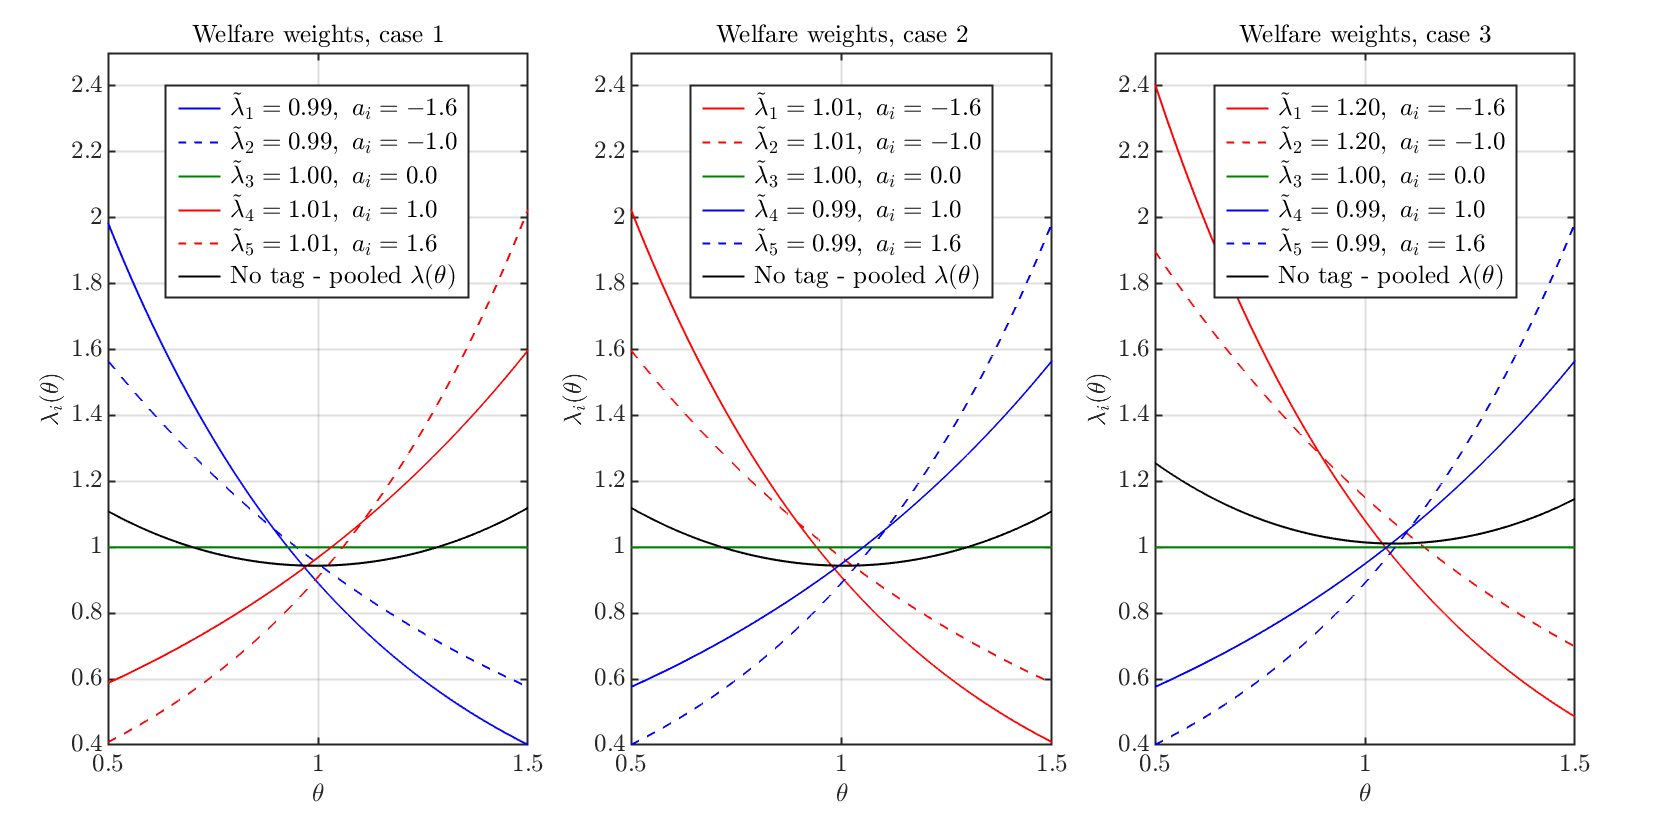
\includegraphics[width=0.9\linewidth]{figure/ImpliementationCRRA_Across_weight_allcases.png}
\end{figure}

\end{frame}
%%%%%%%%%%%%%%%%%%%%%%%%%%%%%%%%%%%%%%%%%%%%%%%%%%%%%%%%%%%%%

\begin{frame}{Across category: spot vs. no tag vs optimal}
    
\begin{figure}
    \centering
    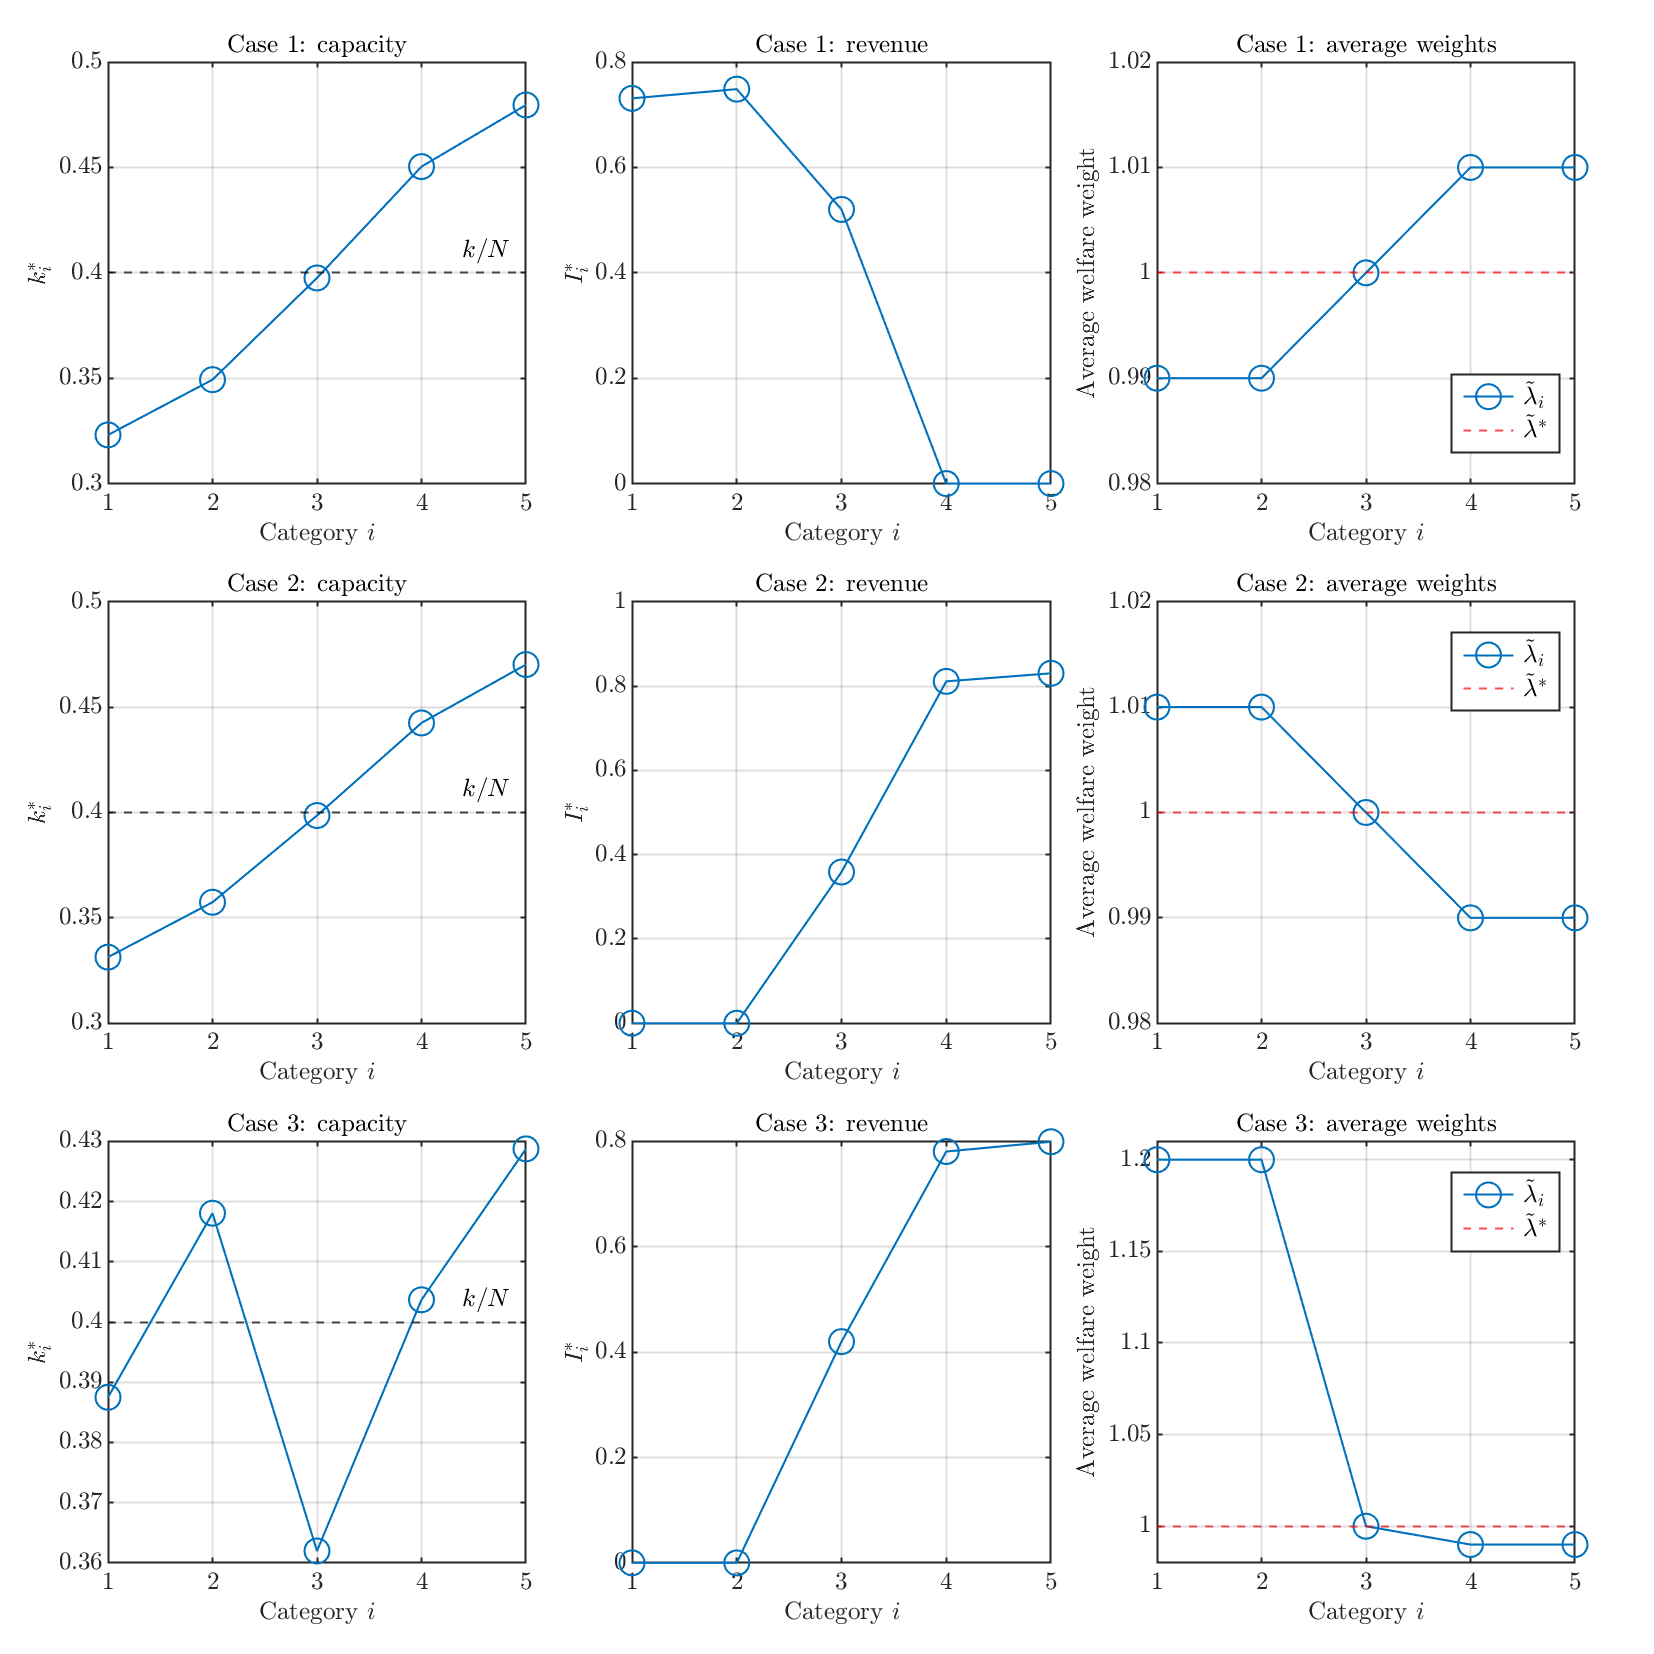
\includegraphics[width=0.5\linewidth]{figure/ImpliementationCRRA_Across_alloc_allcases.png}
\end{figure}
\end{frame}

\end{document}







%%%%%%%%%%%%%%%%%%%%%%%%%%%%%%%%%%%%%%%%%%%%%%%%%%%%%%%%%%%%%